
\chapter{时间相关Hartree-Fock方法\label{chap:tdhf}}

\section{引言\label{sec:12.1}}

在描述原子核中涉及大振幅的过程（例如非简谐振动、裂变与聚变过程）的探索中，迄今为止我们仅使用了定态波函数以及 Ritz 变分原理。

另一方面，我们也可以用时间相关的方式来表述这一问题。设在时间 $t=0$ 时以波函数 $|\Psi(0)\rangle$ 出发，它并不是定态多体
Schrödinger 方程的精确解。这样的态代表一个波包（wave packet），其随时间的演化由时间演化算符给出：

\begin{equation}
|\Psi(t)\rangle=\mathrm{e}^{-\mathrm{i}Ht/\hbar}|\Psi(0)\rangle\label{eq:12.1}
\end{equation}

其中 $H$ 为完整的多体 Hamilton 量。时间相关波函数 $|\Psi(t)\rangle$ 中包含的信息在原理上等价于定态
Schrödinger 方程的解，因为对 $|\Psi(t)\rangle$ 进行 Fourier 分析即可给出 $H$ 的能谱及相应的本征态。另一方面，用波包来描述系统更贴近我们的经典直觉。例如在裂变过程中，我们脑海中会浮现出一个在每个时刻都具有确定形变的经典液滴。在微观图景中，这样一个形变态可由形变势阱中的一个
Slater 行列式来表示，它显然不是 $H$ 的本征态，而是\ref{eq:12.1} 意义上的波包。事实上，我们将会看到，在这样一种图景下，在一定的近似下可以导出经典运动方程。

一般拟设\ref{eq:12.1} 对于实际求解而言显然过于复杂。因此，在本章中，我们将分相继的两步作出明确的近似：

(i) 在时间相关 Hartree-Fock（TDHF）理论中，我们以一个 Slater 行列式 $|\Phi(0)\rangle$
出发，并假设它在所有时刻都保持为 Slater 行列式。一般而言，这是一个极强的近似，正如我们将看到的，这在解释计算结果时会带来严重的问题。另一方面，在静态情形中我们已经看到，这一假设的基础在于：由于
Pauli 原理，每个核子并不与其他核子直接发生相互作用，而仅仅与自洽场的势壁相互作用。结合力通过 Brueckner 理论的重整化，以及通过
HFB 理论对配对关联的计入，该近似在整个元素周期表中对基态和单粒子能级都给出了极佳的描述。至少对于单粒子能量远低于 Fermi 能的情况，Pauli
原理在时间相关情形下也应以类似的方式起作用，没有理由认为 HF 近似在动态情形中会失效。存在着广泛的物理现象（例如低激发集体态、核裂变以及中等能量下的重离子碰撞），在这些现象中这种方法都是合理的。因此，我们将在
\ref{sec:12.2} 节中推导作为该理论基础的 TDHF 方程，并讨论它们的性质和所涉及的问题。我们还将介绍若干应用。自然地，计算中使用了密度依赖的相互作用，并且在许多情况下还必须计入配对关联
\cite{Be66,BF76}。由于进行此类计算的方法是显而易见的，我们在此仅针对不含配对关联（$\rho^{2}=\rho$）的纯
Slater 行列式来展示整个理论。

(ii) 在第二步中，我们采用绝热近似（adiabatic approximation），即假定我们系统中的速度很小。将速度展开到二阶便得到了绝热时间相关
Hartree-Fock（ATDHF）理论。它导出的方程在原理上并不比 TDHF 方程更容易求解，但它为理解物理问题提供了极大的洞察力，并允许对所有可用少数集体变量来描述运动的情形导出一个集体
Hamilton 量。这将在 \ref{sec:12.3} 节中予以讨论。

\section{完整的时间相关Hartree-Fock理论\label{sec:12.2}}

\subsection{TDHF方程的推导\label{subsec:12.2.1}}

我们从任意波包 $|\Psi(0)\rangle$ 出发。其精确时间演化由\ref{eq:12.1} 给出，其在时间 $t$
时的单体密度为

\begin{equation}
\rho_{kl}(t)=\langle\Psi(t)|c^{\dagger}_{l}c_{k}|\Psi(t)\rangle\label{eq:12.2}
\end{equation}

为了得到运动方程，我们计算其对时间的一阶导数：

\begin{equation}
\mathrm{i}\hbar\dot{\rho}_{kl}(t)=\langle\Psi(t)|[c^{\dagger}_{l}c_{k},H]|\Psi(t)\rangle\label{eq:12.3}
\end{equation}

对于两体 Hamilton 量 {[}式 $(5.25)${]}，它可以写为

\begin{equation}
\mathrm{i}\hbar\dot{\rho}_{kl}-\sum_{p}(t_{kp}\rho_{pl}-\rho_{kp}t_{pl})=\frac{1}{2}\sum_{prs}(\bar{v}_{kprs}\rho^{(2)}_{rslp}-\bar{v}_{rslp}\rho^{(2)}_{kprs})\label{eq:12.4}
\end{equation}

其中我们引入了两体密度

\begin{equation}
\rho^{(2)}_{klpq}(t)=\langle\Psi(t)|c^{\dagger}_{p}c^{\dagger}_{q}c_{l}c_{k}|\Psi(t)\rangle\label{eq:12.5}
\end{equation}

我们可以用与\ref{eq:12.3} 中处理单体密度相同的方式来推导这一物理量的运动方程。它将两体密度与三体密度联系起来，以此类推（见附录
F）。这一方程组 \cite{BG49} 是精确的，但显然不是闭合的。为了使其闭合，我们必须引入若干近似。\ref{eq:12.4}
的左端描述了系统的自由运动，仅包含动能项；而右端则包含粒子之间的相互作用。这种相互作用可以划分为两部分：一部分是对所有粒子取平均的自洽单体场；另一部分是无法被平均场所计入的两个核子之间的个别碰撞，后者引起了两体关联。

为了实现这种分解，我们通过从 $\rho^{(2)}$ 中扣除无关联对来定义关联函数 $g^{(2)}$：

\begin{equation}
\rho^{(2)}_{klpq}=\rho_{kp}\rho_{lq}-\rho_{kq}\rho_{lp}+g^{(2)}_{klpq}\label{eq:12.6}
\end{equation}

从而代替\ref{eq:12.4}，得到

\begin{equation}
\mathrm{i}\hbar\dot{\rho}_{kl}-[t+\Gamma,\rho]_{kl}=\frac{1}{2}\sum_{prs}(\bar{v}_{kprs}g^{(2)}_{rslp}-\bar{v}_{rslp}g^{(2)}_{kprs})\label{eq:12.7}
\end{equation}

其中密度依赖的 HF 势为

\begin{equation}
\Gamma_{kl}=\sum_{pq}\bar{v}_{kqlp}\rho_{pq}\label{eq:12.8}
\end{equation}

它与静态 HF 理论 {[}式 $(5.34)${]} 中的定义相同。唯一的区别在于它现在包含精确的时间相关密度 $\rho(t)$；因此，自洽场
$\Gamma$ 是时间相关的。

系统中的粒子现在可以经历两种相互作用：与自洽场 $\Gamma$ 的运动势壁发生碰撞，或者与其他粒子发生碰撞。这两种类型都会给系统带来内部激发。因此，我们必须区分由与势壁碰撞所引起的“单体摩擦（one-body
friction）”（见 \cite{MSK77}），以及由\ref{eq:12.7} 右端的两体碰撞所引起的“两体摩擦（two-body
friction）”。

正如我们在引言中所讨论的，在静态情形下，由于 Pauli 原理，两体关联可以忽略。它们可以被归并到 Brueckner 理论中经适当重整化的有效相互作用中。因此我们同样预期，在动态情形下，只要每个粒子的激发能量低于
Fermi 能，$g^{(2)}$ 便可以忽略，两体散射不会起主要作用。在经典极限（$\hbar\to0$）下，这对应于忽略 Boltzmann
方程中的碰撞项，我们将在第 13 章中更详细地讨论这一点。在此情形下，\ref{eq:12.6} 中的两体密度 $\rho^{(2)}$
发生因式分解，可以完全用单体密度 $\rho$ 来表示；于是波函数 $|\Psi(t)\rangle$ 在所有时刻都保持为 Slater
行列式 $|\Phi(t)\rangle$。令 $g^{(2)}=0$，我们最终得到了 TDHF 方程 \cite{Di30}：

\begin{equation}
\mathrm{i}\hbar\dot{\rho}=[h,\rho]\label{eq:12.9}
\end{equation}

其中 $h=t+\Gamma$。这是关于单体密度矩阵 $\rho$ 的非线性矩阵方程，也是关于时间的一阶微分方程。从初始条件 $\rho(0)$
出发，它确定了所有时刻的 $\rho(t)$。\footnote{此方程在核物理中首次由 Ferrell \cite{Fe57} 明确使用。}

在存在外场 $F(t)=\sum_{kl}f_{kl}(t)c^{\dagger}_{k}c_{l}$ 的情况下，对应的 Schrödinger
方程为

\begin{equation}
\mathrm{i}\hbar|\dot{\Psi}(t)\rangle=(H+F(t))|\Psi(t)\rangle\label{eq:12.10}
\end{equation}

即我们必须将\ref{eq:12.3} 中的 Hamilton 量 $H$ 替换为 $H+F(t)$，或者将\ref{eq:12.9}
中的矩阵 $h$ 替换为 $h+f(t)$。这曾被用来推导时间相关外场中的线性响应理论（见 8.5 节）。

在坐标空间中（引入自旋和同位旋变量的方法是显而易见的），对于自旋无关的两体势 $v(\boldsymbol{r},\boldsymbol{r}')$，TDHF
方程 \ref{eq:12.9} 具有如下形式：

\begin{align}
\mathrm{i}\hbar\dot{\rho}(\boldsymbol{r},\boldsymbol{r}',t) & =-\frac{\hbar^{2}}{2m}(\Delta_{\boldsymbol{r}}-\Delta_{\boldsymbol{r}'})\rho(\boldsymbol{r},\boldsymbol{r}',t)+(\Gamma_{H}(\boldsymbol{r})-\Gamma_{H}(\boldsymbol{r}'))\rho(\boldsymbol{r},\boldsymbol{r}',t)\nonumber \\
 & \quad+\int\mathrm{d}^{3}r''\left(\Gamma_{\text{Ex}}(\boldsymbol{r},\boldsymbol{r}'')\rho(\boldsymbol{r}'',\boldsymbol{r}',t)-\Gamma_{\text{Ex}}(\boldsymbol{r}'',\boldsymbol{r}')\rho(\boldsymbol{r},\boldsymbol{r}'',t)\right)\label{eq:12.11}
\end{align}

其中 $\Gamma_{H}$ 和 $\Gamma_{\text{Ex}}$ 的定义见式 $(5.42)$ 及后文。

我们看到，如果我们将 Slater 行列式 $|\Phi(0)\rangle$ 分解为 $A$ 个相互正交的单粒子波函数 $\varphi_{i}(\boldsymbol{r},0)\;(i=1,\dots,A)$，并通过单粒子波函数的
TDHF 方程追踪它们的时间演化：

\begin{equation}
\mathrm{i}\hbar\frac{\partial}{\partial t}\varphi_{i}(\boldsymbol{r},t)=\left(-\frac{\hbar^{2}}{2m}\Delta+\Gamma_{H}(\boldsymbol{r},t)\right)\varphi_{i}(\boldsymbol{r},t)+\int\mathrm{d}^{3}r'\Gamma_{\text{Ex}}(\boldsymbol{r},\boldsymbol{r}',t)\varphi_{i}(\boldsymbol{r}',t)\label{eq:12.12}
\end{equation}

则我们可以得到\ref{eq:12.9} 的一个解 $\rho(t)$。密度 $\rho$ 随后由下式给出：

\begin{equation}
\rho(\boldsymbol{r},\boldsymbol{r}',t)=\sum^{A}_{i=1}\varphi_{i}(\boldsymbol{r},t)\varphi^{*}_{i}(\boldsymbol{r}',t)\label{eq:12.13}
\end{equation}

TDHF 方程的这种形式在实际计算中更易于处理，因为求解依赖于四个坐标 $(\boldsymbol{r},t)$ 的 $A$ 个微分方程，要比求解像\ref{eq:12.11}
那样依赖于七个坐标 $(\boldsymbol{r},\boldsymbol{r}',t)$ 的单个微分方程更为简便。

在讨论 TDHF 方程的性质之前，我们应当指出，它也可以从时间相关变分原理中导出 \cite{KK76}。Lagrange 量定义为

\begin{equation}
\mathcal{L}=\left\langle \Phi(t)\left|\mathrm{i}\hbar\frac{\partial}{\partial t}-H\right|\Phi(t)\right\rangle \label{eq:12.14}
\end{equation}

在 $|\Phi(t)\rangle$ 是单粒子波函数 $\varphi_{1}(\boldsymbol{r},t),\dots,\varphi_{A}(\boldsymbol{r},t)$
的 Slater 行列式\footnote{此变分原理可以被推广。若 $|\Phi\rangle$ 是一个一般的多体波函数，则可以导出精确的 Schrödinger 方程 \cite{KK76}。}的假设下，$\mathcal{L}$
是 $2A$ 个独立场量 $\varphi_{i}(\boldsymbol{r},t)$ 与 $\varphi^{*}_{i}(\boldsymbol{r},t)$
的泛函。将它们视为经典场变量，我们可以在固定的端点 1 和 2 之间定义一个作用量

\begin{equation}
I_{12}=\int^{t_{2}}_{t_{1}}\mathcal{L}[\boldsymbol{\varphi},\boldsymbol{\varphi}^{*}]\,\mathrm{d}t\label{eq:12.15}
\end{equation}

Hamilton 变分原理 \cite{Go59}

\begin{equation}
\delta I_{12}=0\label{eq:12.16}
\end{equation}

对 $\boldsymbol{\varphi}$ 与 $\boldsymbol{\varphi}^{*}$ 进行独立变分，便给出了运动方程
\ref{eq:12.12}。

\subsection{TDHF方程的性质\label{subsec:12.2.2}}

\subsubsection{乘积特性的守恒\label{subsubsec:12.2.2.1}}

在前一节中，我们假设波函数 $|\Phi(t)\rangle$ 在所有时刻都是 Slater 行列式，并在此条件下导出了 TDHF
方程 \ref{eq:12.9}。因此，我们首先必须证明该理论是自洽的，也就是说，如果我们从 Slater 行列式的密度（$\rho^{2}(0)=\rho(0)$）出发，这一性质在所有时刻都是守恒的：

\begin{equation}
\mathrm{i}\hbar\frac{\partial}{\partial t}(\rho^{2}-\rho)=\mathrm{i}\hbar(\dot{\rho}\rho+\rho\dot{\rho}-\dot{\rho})=[h,\rho^{2}-\rho]\label{eq:12.17}
\end{equation}

在第 7 章中，我们详细讨论了当所有 Slater 行列式以适当方式参数化时所得到的能量曲面。因此，TDHF 方程的解 $|\Phi(t)\rangle$
对应于该能量曲面上的一条轨迹。

\subsubsection{正交性的守恒\label{subsubsec:12.2.2.2}}

与刚刚讨论的性质密切相关的事实是：单粒子波函数 $\varphi_{i}(\boldsymbol{r},t)$ 在所有时刻都保持正交：

\begin{equation}
\mathrm{i}\hbar\frac{\partial}{\partial t}\langle\varphi_{i}|\varphi_{k}\rangle=\langle\varphi_{i}|h-h^{\dagger}|\varphi_{k}\rangle=0\label{eq:12.18}
\end{equation}


\subsubsection{对称性算符期望值的守恒\label{subsubsec:12.2.2.3}}

对于任意与时间无关的单粒子算符 $F=\sum f_{lm}c^{\dagger}_{l}c_{m}$，由\ref{eq:12.9}
我们得到在态 $|\Phi(t)\rangle$ 中的期望值满足

\[
\mathrm{i}\hbar\frac{\mathrm{d}}{\mathrm{d}t}\langle F\rangle=\mathrm{i}\hbar\mathrm{Tr}(f\cdot\dot{\rho})=\mathrm{Tr}(f\cdot[h,\rho])
\]

或

\begin{equation}
\mathrm{i}\hbar\frac{\mathrm{d}}{\mathrm{d}t}\langle F\rangle=\langle[F,H]\rangle\label{eq:12.19}
\end{equation}

其中最后一个期望值是利用 Wick 定理（见 C.4 节）计算的。因此，我们发现 Hamilton 量的所有对称性至少在平均意义上都是守恒的。例如：

(i) 粒子数：$(\mathrm{d}/\mathrm{d}t)\langle N\rangle=(\mathrm{d}/\mathrm{d}t)\mathrm{Tr}\rho=0$，式
$(12.20)$；

(ii) 总线动量：$(\mathrm{d}/\mathrm{d}t)\langle\boldsymbol{P}\rangle=0$，式
$(12.21)$；

(iii) 总角动量：$(\mathrm{d}/\mathrm{d}t)\langle\boldsymbol{J}\rangle=0$，式
$(12.22)$。

然而，这并不意味着 $|\Phi\rangle$ 必须是这些对称性算符的本征态。例如，任何定域的密度分布 $\rho(\boldsymbol{r})$
都破坏了平移不变性。我们将在 \ref{subsubsec:12.2.2.5} 节中讨论对称性守恒的问题。

此外，由\ref{eq:12.19}，对于速度无关的相互作用，对于质心 $\boldsymbol{R}=(1/A)\sum\boldsymbol{r}_{i}$
我们得到

\begin{equation}
\frac{\mathrm{d}}{\mathrm{d}t}\langle\boldsymbol{R}\rangle=\frac{1}{Am}\langle\boldsymbol{P}\rangle\label{eq:12.23}
\end{equation}


\subsubsection{能量守恒\label{subsubsec:12.2.2.4}}

能量对时间的全导数可以用密度的变化来表示。由于 $\rho$ 始终保持为 Slater 行列式，在使 $\rho$ 对角化的基底中
$\dot{\rho}$ 仅具有 $ph$ 矩阵元（见 5.3.3 节）：

\begin{equation}
\frac{\mathrm{d}}{\mathrm{d}t}\langle H\rangle=\frac{\mathrm{d}}{\mathrm{d}t}E=\sum_{mi}\left(\frac{\partial E}{\partial\rho_{mi}}\dot{\rho}_{mi}+\frac{\partial E}{\partial\rho_{im}}\dot{\rho}_{im}\right)=\mathrm{Tr}(h\dot{\rho})=\frac{\mathrm{i}}{\hbar}\mathrm{Tr}(h\cdot[\rho,h])=0\label{eq:12.24}
\end{equation}

这意味着能量随时间是守恒的。因此，运动必须在 Slater 行列式的多维能量曲面的等能线上进行。因而，如果我们的初始条件位于某个势谷内，使得能量小于该势谷周围最低的鞍点能量，系统就永远无法离开该势谷。系统将在势谷内的等势线上运行。

在 5.4 节中，我们讨论了 Lipkin 模型中这样一个能量曲面的例子。这里的 HF 能量 $\langle H\rangle$
依赖于两个变量 $\alpha$ 和 $\varphi$。可以将它们变换为一个坐标和正则共轭动量，使得 TDHF 方程成为相应相空间中的经典运动方程
\cite{KLD80}。

\subsubsection{自洽对称性\label{subsubsec:12.2.2.5}}

在 \ref{subsubsec:12.2.2.3} 节中我们看到，精确 Hamilton 量 $H$ 的对称性与相应算符期望值的守恒定律相联系。任何平均场理论的基本特征之一在于波函数和密度可以破坏这些对称性。随着时间的推移，原子核的形变或位置可能会发生剧烈的改变。

然而，正如我们在静态情形中所见到的，可能存在自洽对称性（见 5.5 节）。它们在动态情形中同样会出现：若 $S$ 为一个与 Hamilton
量 $H$ 以及初始密度 $\rho(0)$ 均对易的幺正对称性操作，则 $\rho$ 在所有时刻在该操作下都保持不变。令 $\bar{\rho}=S\rho S^{\dagger}$，我们得到

\begin{equation}
\mathrm{i}\hbar\frac{\partial}{\partial t}(\bar{\rho}-\rho)=[h(\bar{\rho})-h(\rho),\bar{\rho}]+[h(\rho),\bar{\rho}-\rho]\label{eq:12.25}
\end{equation}

即若在时刻 $t$ 对称性是守恒的（$\bar{\rho}=\rho$），则在时刻 $t+\mathrm{d}t$ 它也是守恒的。

这一事实具有数值上的优势，因为可以减小矩阵的维数。然而，在施加对称性时，我们极大地限制了可能的运动，并阻碍了许多关联的发展。即使在对称性破缺对原子核的宏观形状影响不大的情况下，内部的单粒子运动也可能发生剧烈改变，因为自洽对称性限制了每个单独单粒子轨道的自由度。例如在轴对称的情形下，每个核子都必须平行或反平行于对称轴顺排，从而统计涨落受到抑制。换句话说，固定的势壁不会加热系统，为了获得完整的单体耗散（one-body
dissipation），我们必须破缺所有可能的对称性。

若在解 $\rho(t)$ 中破缺了某个连续对称性，正如在静态情形中那样，仅通过施加该对称性操作，我们就能得到无穷多个其他的解。坐标系的平移就是一个例子。

\subsubsection{时间反演不变性\label{subsubsec:12.2.2.6}}

作为 TDHF 方程 \ref{eq:12.9} 动力学解的密度分布 $\rho(t)$ 不是时间反演不变的，其意义在于时间反演算符
\cite[第十五章]{Me61}

\begin{equation}
T=K_{0}\mathrm{e}^{-\mathrm{i}\pi s_{y}}\label{eq:12.26}
\end{equation}

（其中 $K_{0}$ 为复共轭算符）会改变 $\rho$：

\begin{equation}
\rho_{T}(t):=T\rho(t)T^{\dagger}\neq\rho(t)\label{eq:12.27}
\end{equation}

因为 $\rho_{T}=\rho$ 将要求 $\dot{\rho}=0$。另一方面，我们具有微观可逆性（microscopic
reversibility），这意味着 $\rho_{T}(-t)$ 也是 TDHF 方程的一个解。事实上，这一性质常被用来检验求解\ref{eq:12.9}
的计算机程序的精度。然而，这仅仅是微观可逆性，并不意味着系统（在该理论范围内）不能被加热。

\subsection{准静态解\label{subsec:12.2.3}}

\subsubsection{平移\label{subsubsec:12.2.3.1}}

正如我们在上一节中所见，TDHF 方程的动力学解不可能完全是时间偶的。在特殊情况下，我们已经可以通过破坏时间反演对称性的适当变换，从静态
HF 方程的解中求得该方程的动力学解。

此类情形的一个简单例子是变换到以恒定速度 $\boldsymbol{v}$ 运动的参考系的 Galilei 变换。它由算符 $G$
实现（见 \cite[第十五章]{Me61}）：

\begin{equation}
G(\boldsymbol{v},t)=\exp\left(-\frac{\mathrm{i}}{\hbar}\boldsymbol{v}\cdot(mA\boldsymbol{R}-\boldsymbol{P}t)\right)\label{eq:12.28}
\end{equation}

其中 $\boldsymbol{R}=(1/A)\sum\boldsymbol{r}_{i}$ 为质心坐标，$\boldsymbol{P}=\sum\boldsymbol{p}_{i}$
为总动量。与该变换相对应的是单粒子空间中的一个矩阵：$g(\boldsymbol{v},t)=\exp[-(\mathrm{i}/\hbar)\boldsymbol{v}\cdot(m\boldsymbol{r}-\boldsymbol{p}t)]$，它变换密度矩阵：

\begin{equation}
\rho(t)\to\bar{\rho}=g\rho(t)g^{\dagger}\label{eq:12.29}
\end{equation}

$\bar{\rho}$ 满足运动方程

\begin{equation}
0=\mathrm{i}\hbar\dot{\bar{\rho}}=g[h,\rho]g^{\dagger}-g[\boldsymbol{v}\cdot\boldsymbol{p},\rho]g^{\dagger}=[h(\bar{\rho})-\boldsymbol{v}\cdot\boldsymbol{p},\bar{\rho}]\label{eq:12.30}
\end{equation}

利用\ref{eq:12.28} 以及对于速度无关和平移不变相互作用成立的对称性性质 $g\Gamma(\rho)g^{\dagger}=\Gamma(\bar{\rho})$，我们在运动参考系中再次找到了
TDHF 方程：

\begin{equation}
0=\mathrm{i}\hbar\dot{\bar{\rho}}=\left[\frac{1}{2m}(\boldsymbol{p}+m\boldsymbol{v})^{2}+\Gamma(\bar{\rho})-\boldsymbol{v}\cdot(\boldsymbol{p}+m\boldsymbol{v}),\bar{\rho}\right]=[h(\bar{\rho}),\bar{\rho}]\label{eq:12.31}
\end{equation}

由此我们看到，运动参考系中的静态解 $[h(\bar{\rho}),\bar{\rho}]=0$ 变换成了实验室参考系中 TDHF
方程的非平凡动力学解。它具有如下形式：

\begin{equation}
\rho(t)=\mathrm{e}^{(\mathrm{i}/\hbar)m\boldsymbol{v}\cdot\boldsymbol{r}}\left(\mathrm{e}^{-(\mathrm{i}/\hbar)\boldsymbol{v}\cdot\boldsymbol{p}t}\bar{\rho}\mathrm{e}^{(\mathrm{i}/\hbar)\boldsymbol{v}\cdot\boldsymbol{p}t}\right)\mathrm{e}^{-(\mathrm{i}/\hbar)m\boldsymbol{v}\cdot\boldsymbol{r}}\label{eq:12.32}
\end{equation}

这表明定态解 $\bar{\rho}$ 首先经历坐标的时间偶平移量 $-\boldsymbol{v}t$，然后通过动量的时间奇变换获得一个速度。在坐标空间中，我们得到

\begin{equation}
\rho(\boldsymbol{r},\boldsymbol{r}',t)=\mathrm{e}^{(\mathrm{i}/\hbar)m\boldsymbol{v}\cdot(\boldsymbol{r}-\boldsymbol{r}')}\cdot\mathrm{e}^{-\boldsymbol{v}t\cdot(\boldsymbol{\nabla}_{\boldsymbol{r}}+\boldsymbol{\nabla}_{\boldsymbol{r}'})}\bar{\rho}(\boldsymbol{r},\boldsymbol{r}')\label{eq:12.33}
\end{equation}

在时刻 $t=0$ 时，对角密度 $\rho(\boldsymbol{r},\boldsymbol{r},0)$ 与定态值 $\bar{\rho}$
完全相同。集体速度仅通过非对角部分中依赖于 $\boldsymbol{r}$ 的相位因子表现出来。

在 TDHF 理论应用于重离子反应的实际计算中，人们通常采用两个形如\ref{eq:12.33} 且速度分别为 $\boldsymbol{v}_{1}$
和 $\boldsymbol{v}_{2}$、相隔距离足够远而不发生重叠的密度之和作为初始条件。在很好的近似下，它们代表在反应发生之前处于基态的两个运动离子。

\subsubsection{转动\label{subsubsec:12.2.3.2}}

在转动的情形下，我们也希望变换到一个转动参考系，在该参考系中运动可以用静态解来描述。然而与平移不同，转动集体运动是非平凡的。在此种情形下不存在“质心角”，也不存在
Galilei 不变性（见 11.3.3 节）。尽管如此，我们可以执行变换 \ref{eq:12.28} 的第一部分，即将坐标变换到以角速度
$\boldsymbol{\omega}$ 转动的参考系：

\begin{equation}
\tilde{\rho}=\mathrm{e}^{\mathrm{i}\boldsymbol{\omega}\cdot\boldsymbol{j}t}\rho(t)\mathrm{e}^{-\mathrm{i}\boldsymbol{\omega}\cdot\boldsymbol{j}t}\label{eq:12.34}
\end{equation}

类比于\ref{eq:12.30}，我们得到

\begin{equation}
\mathrm{i}\hbar\dot{\tilde{\rho}}=\mathrm{e}^{\mathrm{i}\boldsymbol{\omega}\cdot\boldsymbol{j}t}[t+\Gamma(\rho)-\boldsymbol{\omega}\cdot\boldsymbol{j},\rho]\mathrm{e}^{-\mathrm{i}\boldsymbol{\omega}\cdot\boldsymbol{j}t}=[h(\tilde{\rho})-\boldsymbol{\omega}\cdot\boldsymbol{j},\tilde{\rho}]\label{eq:12.35}
\end{equation}

现在我们得到了自洽 Cranking 模型的定态 HF 问题（见 7.7 节和 11.4.6.3 节）：

\begin{equation}
[h(\tilde{\rho})-\boldsymbol{\omega}\cdot\boldsymbol{j},\tilde{\rho}]=0\label{eq:12.36}
\end{equation}

它给出了一个不具时间依赖性但包含时间奇分量的密度 $\tilde{\rho}$。在此意义上它并不是静态密度。同样，

\begin{equation}
\rho(t)=\mathrm{e}^{-\mathrm{i}\boldsymbol{\omega}\cdot\boldsymbol{j}t}\tilde{\rho}\mathrm{e}^{\mathrm{i}\boldsymbol{\omega}\cdot\boldsymbol{j}t}\label{eq:12.37}
\end{equation}

是 TDHF 方程 \ref{eq:12.9} 的一个非平凡解。

\ref{eq:12.36} 也可以从投影 TDHF 理论以如下方式更根本地导出 \cite{EMR80b}。类比于\ref{eq:12.14}，我们从
Lagrange 量出发：

\[
\mathcal{L}=\left\langle \Phi(t)\left|\hat{P}^{I}\left(\mathrm{i}\hbar\frac{\partial}{\partial t}-H\right)\hat{P}^{I}\right|\Phi(t)\right\rangle 
\]

其中 $\hat{P}^{I}$ 是好角动量投影算符（见 11.4.6 节）。作用量 \ref{eq:12.15} 对时间相关的
Slater 行列式 $|\Phi(t)\rangle$ 的变分便给出了投影 TDHF 方程。在大形变极限下，我们可以使用一阶 Kamlah
展开 {[}式 $(11.80)${]} 并得到\ref{eq:12.35}。其最简单的解由定态问题 \ref{eq:12.36}
给出。

如果相信 Cranking 模型，人们便可通过这种方式看出：投影在时间相关 HF 情形下是一个非常重要的特征。这在其他问题中也变得显而易见，例如在反应截面的计算中，我们必须向各个反应道进行投影（见
\ref{subsec:12.2.4} 节）。

\subsection{TDHF方法的一般讨论\label{subsec:12.2.4}}

乍看起来，TDHF 方法似乎具有极具吸引力的优势。它为原子核中各类集体运动提供了统一的描述：从基态的静态解出发，历经转动与振动激发，直至大振幅集体运动，诸如裂变、聚变、复合核形成以及深部非弹性反应。系统能够在多维能量曲面上自行决定其演化路径，该能量曲面包含了所有可由乘积态表示的构型。特别地，我们无需先验地选取某些集体坐标，也无需迫使系统在非物理的外场中运动。我们无需预先了解系统内部的流动模式，也无需知道惯性参数及其对坐标的依赖关系。

另一方面，这一概念并不仅仅描述集体现象：在所有时刻波函数都保持为 Slater 行列式。它兼顾了单粒子结构的所有方面，并包含了集体运动与单粒子运动之间的完全相互作用。

最后，TDHF 方程的解还包含了摩擦与阻尼效应，只要这些效应是由粒子与时间相关平均场的势壁相互作用所产生的——即所谓的单体摩擦（one-body
friction，见 \cite{BBN78} 及其所列参考文献）。

为了看清在巨共振情形下这种阻尼的来源，我们利用 Thouless 定理 {[}式 $(\text{E}.26)${]}，在 HF
基态 $|\Phi_{0}\rangle$ 的基底中展开 $|\Phi(t)\rangle$：

\begin{align}
|\Phi(t)\rangle & \propto\exp\left(\sum_{mi}z_{mi}(t)a^{\dagger}_{m}a_{i}\right)|\Phi_{0}\rangle\nonumber \\
 & =|\Phi_{0}\rangle+\sum_{mi}z_{mi}(t)a^{\dagger}_{m}a_{i}|\Phi_{0}\rangle+\sum_{mim^{\prime}i^{\prime}}z_{mi}(t)z_{m^{\prime}i^{\prime}}(t)a^{\dagger}_{m}a^{\dagger}_{m^{\prime}}a_{i^{\prime}}a_{i}|\Phi_{0}\rangle+\dots\label{eq:12.38}
\end{align}

我们看到，除了 ph 掺杂（这在第 8 章的 TDA 或 RPA 中已经处理过）之外，TDHF 波函数还包含 2p2h、3p3h 分量等等。为了得到这些掺杂成分随能量变化的强度，我们必须对
$|\Phi(t)\rangle$ 进行 Fourier 变换。

迄今为止，尚不清楚巨共振的扩散宽度\footnote{然而我们应当注意，TDHF 理论包含了正如在 8.5.4 节中所讨论的逃逸宽度（escape width），这意味着粒子实际上正在离开原子核。}中有多少来自此类
2p2h 掺杂（单体摩擦），以及略去\ref{eq:12.7} 中的碰撞项 $I(\rho)$ 或\ref{eq:12.7}
中的 $g^{(2)}$ 项（二体摩擦）在多大程度上是正确的。\ref{eq:12.7} 中 $g^{(2)}$ 项可以忽略的近似，反过来又基于这样一种观点
\cite{KK68}：由于 Pauli 不相容原理，核子的平均自由程与核线度具有相同的数量级。这一假设的有效性在每粒子能量达到
Fermi 能数量级时必然失效，但仍有广泛的现象我们应当能够用 TDHF 方法来描述。

特别地，该理论并不必然受限于绝热假设——即波函数在每一时刻都非常接近相应自洽势阱 $h(t)$ 的基态。对于动态解而言，TDHF
单粒子函数 $\phi_{i}(t)$ {[}\ref{eq:12.12}{]} 与该势阱中的本征函数是不同的：

\begin{equation}
h(t)|\psi_{k}(t)\rangle=\epsilon_{k}(t)|\psi_{k}(t)\rangle\label{eq:12.39}
\end{equation}

这意味着我们并不能通过填满势阱 $h(t)$ 中的最低 $A$ 个能级来获得 TDHF Slater 行列式 $|\Phi(t)\rangle$。密度
$\rho(t)$ 与 $h(t)$ 并不对易，也就是说，$\rho(t)$ 在本征函数 $|\psi_{k}(t)\rangle$
构成的基底中不是对角的，占有几率 $\rho_{k}$（即 $\rho$ 在该基底下的对角元）：

\begin{equation}
\rho_{k}(t)=\langle\psi_{k}(t)|\rho(t)|\psi_{k}(t)\rangle\label{eq:12.40}
\end{equation}

弥散分布在许多能级上，即我们在该基底中得到了一个弥散开的 Fermi 面。另一方面，占有几率的分布也不应过分偏离 Fermi 阶跃函数，即它不应变得完全碎裂，否则不相容原理将不再能够压低二体碰撞。然而，目前对这一问题尚无详细的研究。

尽管 TDHF 方法具有所有这些巨大的优点，但我们必须清醒地认识到该方法存在着某些重要的局限性：

(i) 该理论提供了一种完全微观的描述，它跟踪每个单粒子波函数随时间的变化，因而需要耗费极其巨大的数值计算量。特别地，我们应当牢记：只有当尽可能多的对称性被破缺时，它的全部优势与威力才能展现出来。这种类型的现实计算不仅接近现代计算机算力的极限，而且往往极难从中提取出系统的基本物理特征并借助简明模型加以理解。

(ii) 在某种意义上，该理论表现出经典的确定性行为：我们从一个初始密度 $\rho(t)$ 出发，并在多维能量曲面上跟踪它及其速度
$\dot{\rho}(t)$ 随时间的演化，正如一条经典轨道。仅凭这一事实并不能断言该理论是经典的；精确的量子力学统计算符 $\rho$
服从 von Neumann 方程，其结构与\ref{eq:12.9} 极为相似。与完全量子力学理论的根本差异在于：我们在所有时刻都将波函数限制为
Slater 行列式，从而导出了一个非线性方程。因此我们放弃了态叠加原理，即两个 Slater 行列式的线性组合（一般而言）不再是一个乘积波函数。作为理论非线性的必然结果，我们得到了具有孤子（soliton）特性的解（见
12.2.5 节），即在传播过程中保持形状不变的密度分布 {[}例如见\ref{eq:12.32}{]}，而精确的量子力学密度 $\rho(\boldsymbol{r})=\langle\Psi(t)|\hat{\rho}(\boldsymbol{r})|\Psi(t)\rangle$
必然会表现出通常的量子力学波包弥散。以恒定速度运动的静态密度这一例子 {[}\ref{eq:12.32}{]} 不出现弥散的事实，也可以表述为我们在
TDHF 理论中破坏了平移不变性，即我们处于原子核的内禀参考系中，并将核质心坐标与其动量视为两个可同时测量的（经典）量。这当然与将
Slater 行列式视为精确波函数的近似紧密相关。

(iii) 另一个量子力学效应是穿透势垒的隧道效应。如果我们在能量曲面上有两个分离的局域极小值，并且我们从一个谷中以小于两极小值间最低鞍点的能量出发，由于能量守恒
{[}\ref{eq:12.24}{]}，系统将永远无法到达另一个谷。存在两个不同的谷正是非线性的结果。线性理论永远只有一个极小值，即基态（见
5.2 节）。隧道效应的不可能性在将一般 Slater 行列式集合限制为具有少数集体自由度的乘积波函数 $|\Phi(q)\rangle$
的情形下（见 12.3.3 节，如裂变过程的描述）变得尤为明显。在此类情形中，我们必须要么重新量子化，要么引入乘积态的线性叠加。这把我们带回了生成坐标法（第
10 章）。

在 Slater 行列式空间中的势垒（最终过渡为集体坐标下的势垒），不应与坐标空间中外场 $V(\boldsymbol{r})$
的势垒相混淆。例如，让我们研究一个以确定速度朝向此类外势垒运动的静态解。该系统的波函数 $|\Phi\rangle$ 由单粒子波函数
$\phi_{i}(\boldsymbol{r})$ 的乘积构成。其中每一个波函数都有一个穿透势垒的尾巴。因此一般而言，$|\Phi\rangle$
在该势垒处分裂为两部分：透射部分与反射部分。这两部分各自单独来看都不再是 Slater 行列式，且单粒子波函数 $\phi_{i}$
同时属于这两部分。取决于入射能量，透射与反射部分具有非常不同的大小。\ref{fig:12.1}(a) 给出了在一维计算中的结果，其中一块核物质厚板以每核子能量等于势垒高度的动能向高斯形势垒运动。我们看到整块厚板全部被透射过去。如果没有粒子间通过平均场的相互作用，我们本预期每个单粒子波函数的透射几率仅为
0.5。然而，自洽场与外势垒共同作用，为粒子提供了一个急剧减小的有效势垒。\ref{fig:12.1}(b) 给出了在更高势垒下的同一过程。此时初始厚板分裂为两部分。我们再次观察到，集体穿透几率远高于单个粒子的穿透几率。

\begin{figure}[H]
\begin{centering}
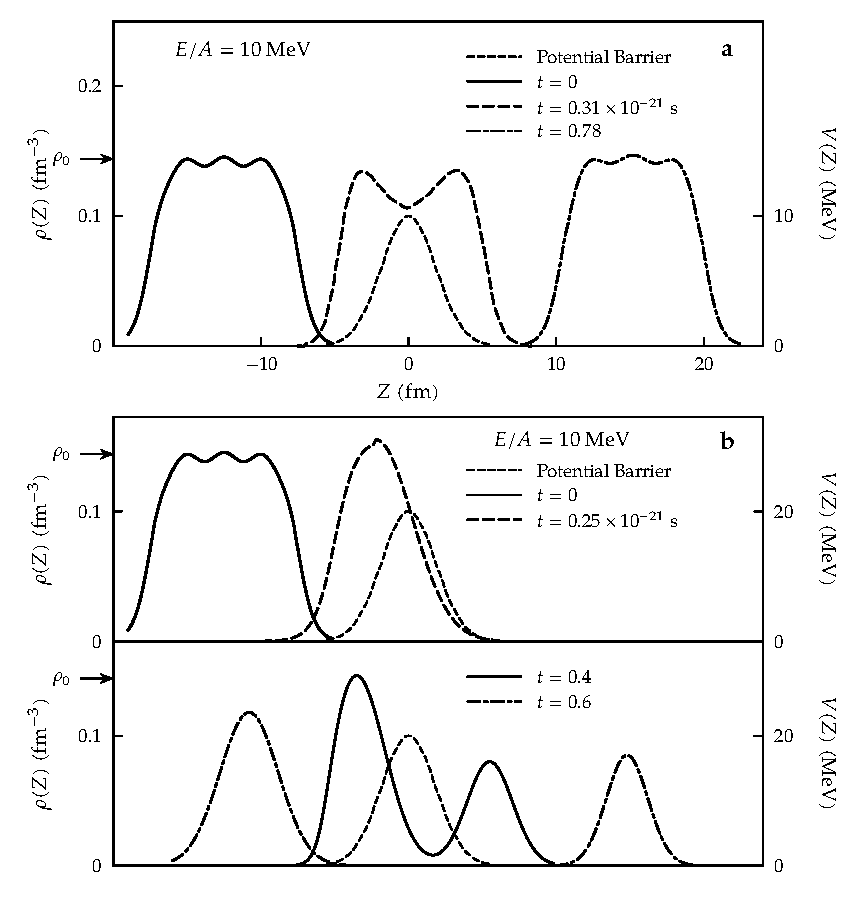
\includegraphics[width=0.85\textwidth]{pictures/12_1}
\par\end{centering}
\caption{\label{fig:12.1}核物质厚板与高度为 10 MeV (a) 和 20 MeV (b) 的高斯势垒的相互作用。（引自
\cite{BKN76}）}
\end{figure}

(iv) 在对波函数 $|\Phi(t)\rangle$ 所包含结果的物理解释中存在着根本性问题。这已经在厚板朝向外势垒运动的例子中显现出来：整块厚板是以某种几率完全穿透，还是在每次碰撞中都碎裂为两个独立的部分，其质量对应于势垒左右两侧积分密度
$|\phi_{i}|^{2}$？在后一种情形下，我们将在每个部分中得到非整数的粒子数，因为正如我们所指出的，散射后的碎片自身不再是
Slater 行列式；从而单粒子波函数同时归属于所有碎片。我们还可以设想这两种可能性的复杂混合。在物理上，我们感兴趣的是 $A_{1}$
个粒子透射而 $A_{2}=A-A_{1}$ 个粒子被反射的几率，即在 $t\to\infty$ 的极限下势垒左侧有 $A_{2}$
个粒子而右侧有 $A_{1}$ 个粒子的几率：

\begin{equation}
P_{A_{1}A_{2}}=\frac{(A_{1}+A_{2})!}{A_{1}!A_{2}!}\int^{\infty}_{0}\mathrm{d}x_{1}\dots\mathrm{d}x_{A_{1}}\int^{0}_{-\infty}\mathrm{d}x_{A_{1}+1}\dots\mathrm{d}x_{A}|\Phi(x_{1}\dots x_{A},t\to\infty)|^{2}\label{eq:12.41}
\end{equation}

这是计算质量分布的一个实用处方，它也已被应用于重离子碰撞的计算中 \cite{Ke76}。

然而在一般情形下，我们希望知道此类反应中不同反应道的 $S$ 矩阵元。能否从 TDHF 计算中获取此类信息是一个悬而未决的问题。原则上，我们可以将
TDHF 方程的波包 $|\Phi(t)\rangle$ 视为精确波包 $|\Psi(t)\rangle$ 的有效近似，从而完全像拥有
$|\Psi(t)\rangle$ 时那样从 $|\Phi(t)\rangle$ 获取 $S$ 矩阵元；例如，我们可以将 $|\Phi\rangle$
投影到模型散射态上。然而，这将意味着计算两个不同多体波函数的重叠，这可能导致极为严重的错误结果，正如下面的考量所示：假设我们计算两个仅有极微小差别的乘积波函数的重叠，其中一个行列式中的所有单粒子波函数与另一个行列式中的波函数处处相差一个微小量
$\epsilon$：

\begin{equation}
(1-\epsilon)^{A}\simeq\mathrm{e}^{-\epsilon A}\label{eq:12.42}
\end{equation}

即对于大粒子数，重叠指数式地微小。如果我们希望计算（例如）静态 HF 波函数与精确波函数的重叠，情况也是如此，其中我们可以假设由于关联效应，每个单粒子轨道以几率
$\epsilon$ 被耗尽（depleted）\cite{Ne77}。尽管 HF 波函数与精确波函数的重叠极小，我们在结合能等方面却依然能获得极佳的结果。这是因为在那里我们只需要计算单体和二体算符的期望值，它至多只涉及两个单粒子波函数。同样的考量在时间相关情形下也成立：从
$|\Phi(t)\rangle$ 计算 $S$ 矩阵元（见上文）意味着在重离子反应情形下我们要计算 $A$ 体算符的期望值（全部
$A$ 个核子的构型均发生了改变），因此这很可能给出相当不可靠的结果。所以在时间相关情形下，我们也必须将自己限制在计算少体算符（诸如粒子数分布、平均能量损失和动量转移）的均值及其涨落上。

与上述问题密切相关的是：从一个 Slater 行列式作为初始条件出发，精确波函数 $|\Psi(t)\rangle$ 在时间演化过程中是否能够保持接近于一个
Slater 行列式。为此，Lichtner 和 Griffin \cite{LG76a} 研究了如下函数的时间相关性：

\begin{equation}
D(t)=\frac{1}{A}\mathrm{Tr}(\rho(t)-\rho^{2}(t))\label{eq:12.43}
\end{equation}

在 $t=0$ 时以 Slater 行列式 $|\Phi_{0}\rangle$ 出发，在短时间内我们发现：

\begin{equation}
D(t)=\left(\frac{t}{\tau}\right)^{2}+\dots\label{eq:12.44}
\end{equation}

其寿命有一个极限：

\begin{equation}
\frac{1}{\tau}\geqslant\frac{2}{\hbar}\sqrt{\frac{1}{A}\left(\langle\Phi_{0}|H^{2}|\Phi_{0}\rangle-\langle\Phi_{0}|H|\Phi_{0}\rangle^{2}\right)}\label{eq:12.45}
\end{equation}

它与函数 $|\Phi_{0}\rangle$ 中每核子的能量弥散成正比。对于真实核，我们发现 $\tau$ 的值在 $10^{-22}$
到 $10^{-21}$ 秒之间。这意味着仅仅在极短的时间之后，波函数 $|\Psi(t)\rangle$ 就已经看起来与 Slater
行列式大相径庭。这再次表明：一旦 $|\Psi(t)\rangle$ 与 $|\Phi(t)\rangle$ 出现微小偏差，重叠
$\langle\Psi(t)|\Phi(t)\rangle$ 就会变得极小；但这并不意味着 $|\Phi(t)\rangle$
不能用于计算少体算符的期望值。

(v) 也许 TDHF 理论中最严重的问题是末态赝相互作用（spurious final state interaction）。在精确计算中，我们将拥有许多不同的出射道，它们在
$t\to\infty$ 时彼此不发生相互作用。在我们厚板朝向势垒运动的例子中，我们可以考虑（例如）穿透一个、两个或三个粒子，而其余粒子被反射。通常，透射系统将具有不同的速度。然而在
TDHF 理论内部，所有反应道都被束缚在势垒右侧的一个共同平均势阱中。为了留在该势阱内，所有反应道都必须持久地交换动量。因此在长时间演化后，我们在不同反应道之间也得到了非物理的赝相互作用。即使我们不计算
$S$ 矩阵元，我们也无法排除这种末态相互作用会对少体算符的平均值产生虚假贡献。类比于静态 HF 问题中的对称性破坏，我们因此应当对各个反应道进行某种投影后变分（见第
11 章）。TDHF 波函数 $|\Phi(t)\rangle$ 必须被理解为一个“内禀”波函数。

事实上，人们可以从精确量子力学传播子的 Feynman 路径积分表象 \cite{FH65} 的鞍点近似中导出 TDHF 方程 \cite{KI77,ER78,NLP79,Re79}，在其中上述问题似乎得到了更为妥善的处理。

\subsection{一个精确可解模型\label{subsec:12.2.5}}

为了研究上述讨论的某些问题，Yoon 和 Negele \cite{YN77} 研究了一个由 $N$ 个玻色子在一维中通过 $\delta$
力相互作用的精确可解模型。\footnote{类似但更为复杂的模型已针对费米子系统被提出 \cite{NW76a,NW78}。}其
Hamilton 量由下式给出：

\begin{equation}
H=-\frac{1}{2}\sum^{N}_{i=1}\frac{\partial^{2}}{\partial x^{2}_{i}}-v\sum^{N}_{i<j=1}\delta(x_{i}-x_{j})\label{eq:12.46}
\end{equation}

该模型对束缚态 \cite{Be31,Mc65} 以及散射态 \cite{Ya67} 都已被精确求解。为了得到所有玻色子在自洽场中占据波函数为
$\phi(x,t)$ 的最低能级的乘积态的时间相关 Hartree 方程，我们使用变分原理\ref{eq:12.16}：

\begin{equation}
\langle\Phi|\mathrm{i}\frac{\partial}{\partial t}-H|\Phi\rangle=N\int\mathrm{d}x\left(\phi^{*}\mathrm{i}\frac{\partial}{\partial t}\phi+\frac{1}{2}\phi^{*}\frac{\partial^{2}}{\partial x^{2}}\phi+\frac{v}{2}(N-1)\phi^{*}\phi^{*}\phi\phi\right)\label{eq:12.47}
\end{equation}

并求得：

\begin{equation}
\mathrm{i}\frac{\partial}{\partial t}\phi+\frac{1}{2}\frac{\partial^{2}}{\partial x^{2}}\phi+v(N-1)\phi^{*}\phi\phi=0\label{eq:12.48}
\end{equation}

其静态解为：

\begin{equation}
\phi_{s}(x)=\frac{\sqrt{(N-1)v}}{2\cosh((N-1)vx/2)}\label{eq:12.49}
\end{equation}

能量为：

\begin{equation}
E_{H}=-\frac{N(N-1)^{2}v^{2}}{24}\label{eq:12.50}
\end{equation}

密度为：

\begin{equation}
\rho_{s}(x)=\frac{N(N-1)v}{4\cosh^{2}((N-1)vx/2)}\label{eq:12.51}
\end{equation}

在 $2N$ 个粒子的动态情形下，\ref{eq:12.48} 具有双孤子解 \cite{ZS72,Do76}（关于孤子的定义与性质，参见综述文章
\cite{SCM73,Ra75}）：

\begin{equation}
\phi(x,t)=\frac{\sqrt{(2N-1)v}}{2}\mathrm{e}^{-(\mathrm{i}/2)(K^{2}-a^{2})t}\frac{\left(\mathrm{e}^{\mathrm{i}Kx}\left\{ \mathrm{e}^{-a(x-Kt)}+\left[K^{2}/(K-\mathrm{i}a)^{2}\right]\mathrm{e}^{-a(3x+Kt)}\right\} \right)+(K\leftrightarrow-K)}{1+2\mathrm{e}^{-2ax}\cosh(2aKt)-2a^{2}\mathrm{e}^{-2ax}\mathrm{Re}\left(\mathrm{e}^{2\mathrm{i}Kx}/(K+\mathrm{i}a)^{2}\right)+\left(K^{4}/(K^{2}+a^{2})^{2}\right)\mathrm{e}^{-4ax}}\label{eq:12.52}
\end{equation}

其中 $4a=(2N-1)v$，且 $K$ 为任意实数。它描述了两个相对动量为 $2K$ 的孤波彼此穿过对方的过程。该波函数是在质心参考系中给出的。为了求出其中一个波包参考系中的密度，我们令
$y=x-Kt$ 并得到：

\begin{equation}
\rho(y,t)=2N\cdot|\phi(y,t)|^{2}\underset{t\to\infty}{=}\frac{N(N-\frac{1}{2})v}{4\cosh^{2}((N-\frac{1}{2})vy/2)}\label{eq:12.53}
\end{equation}

对于大 $N$ 值，它与静态密度\ref{eq:12.51} 相一致。我们还可以证明，两波包相互穿透所产生的时间延迟在大 $N$
极限下与精确的时间延迟相符 \cite{Do76}。另一方面，行列式的寿命\ref{eq:12.45} 对于大 $N$ 趋于零。因此，该模型为我们提供了一个范例：源自平均场理论的结果在大系统极限下可能是精确的，即使其波函数与精确波函数的重叠为零。

\subsection{TDHF理论的应用\label{subsec:12.2.6}}

TDHF 理论最早的应用是在小振幅极限下描述围绕静态解 $\rho_{0}$ 的振动。在第 8 章中我们已经看到，将\ref{eq:12.9}
对 $\delta\rho=\rho-\rho_{0}$ 线性化便导出了随机相位近似（RPA）。

在小速度 $\dot{\rho}$ 但大振幅的极限下，我们得到绝热 TDHF 理论（ATDHF）。这将在 12.3 节中连同其应用一起讨论。因此，我们在本节中将局限于
TDHF 方程 \ref{eq:12.9} 的精确数值解。

TDHF 理论已被应用于精确可解模型中。我们在上一小节给出了这样一个范例。另一个例子是 Lipkin 模型 \cite{Kr77,KLD80}。图
5.3 展示了该模型的能量曲面。TDHF 方程的解即为等能线 \cite{KLD80}。

在所有更为现实的计算中 \cite{BKN76,KDM77,CMM78,BGK78,FKW78}，都采用了 Skyrme 型相互作用力。有限力程修正（$t_{1}p^{2}$）被略去，或者在某些情形下被具有有限力程的
Yukawa 力所取代，该力带有特殊的交换部分，使其仅对自洽势的直接项产生贡献。Coulomb 力中的交换项也被略去。这样，\ref{eq:12.12}
仅为一个微分方程，而不是在一般情形下那样的积分微分方程。

为了进一步简化，我们将讨论限制在一维核物质厚板的情形，此时所有单粒子波函数仅依赖于坐标 $z$：

\begin{equation}
\mathrm{i}\hbar\dot{\phi}_{i}(z,t)=\left(-\frac{\hbar^{2}}{2m}\frac{\partial^{2}}{\partial z^{2}}+\Gamma(z,t)\right)\phi_{i}(z,t)=h(z,t)\phi_{i}(z,t)\label{eq:12.54}
\end{equation}

对坐标 $z$ 进行空间离散化得到一个矩阵方程：

\begin{equation}
\mathrm{i}\hbar\dot{\boldsymbol{\phi}}(t)=h(t)\boldsymbol{\phi}(t)\label{eq:12.55}
\end{equation}

最后，对时间 $t$ 也进行离散化。显而易见的推进方式是：

\begin{equation}
\mathrm{i}\hbar\frac{1}{\Delta t}(\boldsymbol{\phi}^{(n+1)}-\boldsymbol{\phi}^{(n)})=h^{(n)}\boldsymbol{\phi}^{(n)}\label{eq:12.56}
\end{equation}

或：

\begin{equation}
\boldsymbol{\phi}^{(n+1)}=\left(1-\frac{\mathrm{i}}{\hbar}\Delta t\cdot h^{(n)}\right)\boldsymbol{\phi}^{(n)}\label{eq:12.57}
\end{equation}

由于 $(1-(\mathrm{i}/\hbar)\Delta t\cdot h^{(n)})$ 不是幺正的，这会导致数值不稳定性。避免这一问题的方法是用下式代替\ref{eq:12.56}：

\begin{equation}
\mathrm{i}\hbar\frac{1}{\Delta t}(\boldsymbol{\phi}^{(n+1)}-\boldsymbol{\phi}^{(n)})=\frac{1}{2}h^{(n)}(\boldsymbol{\phi}^{(n+1)}+\boldsymbol{\phi}^{(n)})\label{eq:12.58}
\end{equation}

或：

\begin{equation}
\boldsymbol{\phi}^{(n+1)}=\frac{1-\frac{\mathrm{i}}{2\hbar}\Delta t\cdot h^{(n)}}{1+\frac{\mathrm{i}}{2\hbar}\Delta t\cdot h^{(n)}}\boldsymbol{\phi}^{(n)}\label{eq:12.59}
\end{equation}

采用时间演化算符的幺正近似（即所谓的 Crank-Nicholson 算符 \cite{CN47}）。然而该方程涉及矩阵求逆，最近将时间演化算符的
Taylor 级数截断至前几项的方法已被证明具有令人满意的精度 \cite{FKW78}。

相互作用力的力常数通过在静态情形下重现核物质性质来确定。为了研究单个厚板的振荡，初始条件选取为：

\begin{equation}
\phi_{i}(\boldsymbol{r},t=0)=\mathrm{e}^{\mathrm{i}S(\boldsymbol{r})}\phi^{0}_{i}(\boldsymbol{r})\label{eq:12.60}
\end{equation}

其中 $\phi^{0}_{i}$ 为静态单粒子波函数。函数 $S(\boldsymbol{r})$ 决定了 $t=0$ 时的速度分布，该速度分布由流密度
$\boldsymbol{j}(\boldsymbol{r},t)$ 的分布所定义：

\begin{equation}
\boldsymbol{v}(\boldsymbol{r},t)=\frac{\boldsymbol{j}(\boldsymbol{r},t)}{\rho(\boldsymbol{r},t)}=\frac{1}{\rho(\boldsymbol{r},t)}\sum^{A}_{i=1}\frac{\hbar}{2m\mathrm{i}}(\phi^{*}_{i}\boldsymbol{\nabla}\phi_{i}-\phi_{i}\boldsymbol{\nabla}\phi^{*}_{i})\label{eq:12.61}
\end{equation}

或：

\begin{equation}
\boldsymbol{v}(\boldsymbol{r},t=0)=\frac{\hbar}{m}\boldsymbol{\nabla}S(\boldsymbol{r})\label{eq:12.62}
\end{equation}

对于 $S(\boldsymbol{r})=\alpha z^{2}$，我们得到 $v(z)=(2\hbar/m)\alpha z$。在此初始条件下，厚板开始振荡。\ref{fig:12.2}展示了对应于呼吸模的此类振动随不同
$\alpha$ 值的变化情况。即使对于很小的 $\alpha$，这些振荡也是非简谐的，并且似乎并不对应于单一频率。对于较大的
$\alpha$ 值，振荡表现出急剧的涨落。最后，当激发过强时，厚板碎裂为碎片（图中未绘出）。

\begin{figure}[H]
\begin{centering}
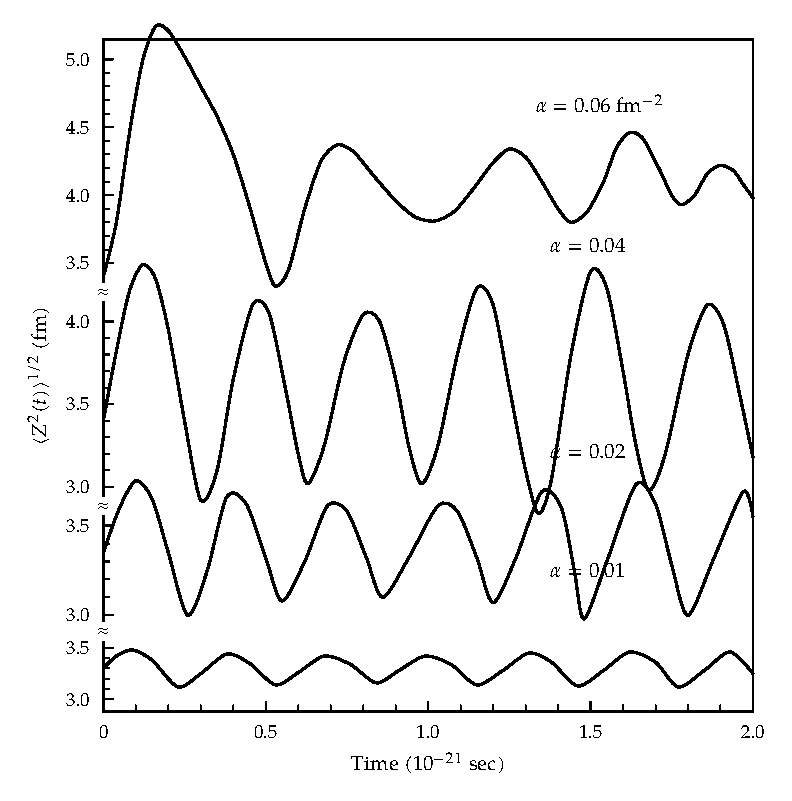
\includegraphics[width=0.8\textwidth]{pictures/12_2}
\par\end{centering}
\caption{\label{fig:12.2}不同初始速度参数 $\alpha$ 下，TDHF 近似中振荡核物质厚板的均方根长度随时间的变化。（引自
\cite{BKN76}）}
\end{figure}

从两个向相反方向运动的自洽厚板出发，我们可以研究碰撞过程。我们发现了丰富多样的现象。取决于入射能量，人们观察到了非弹性散射、复合核形成、共振行为、强阻尼碰撞、转移过程以及碎裂。\ref{fig:12.3}展示了在居中能量下不同时刻的
$\rho(z,t)$。在经历初态聚变后中心密度增加。复合系统开始振荡并在一个周期后发生裂变。

\begin{figure}[H]
\begin{centering}
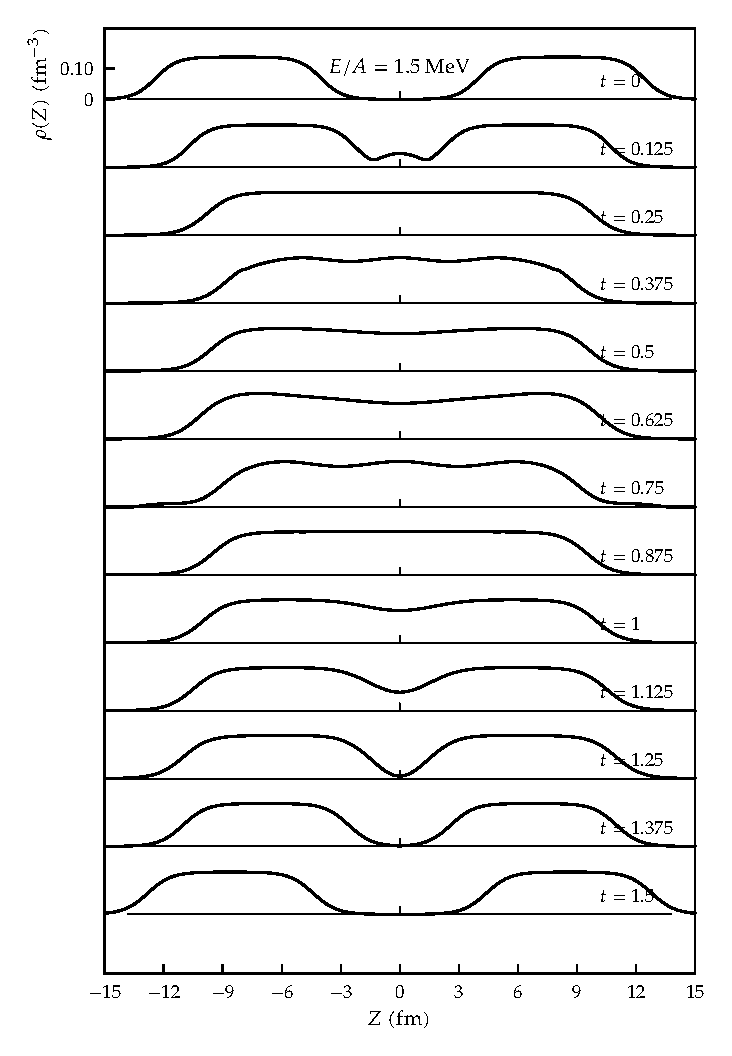
\includegraphics[width=0.75\textwidth]{pictures/12_3}
\par\end{centering}
\caption{\label{fig:12.3}居中能量下两个相同核物质厚板碰撞散射在不同时刻的密度剖面 $\rho(z,t)$。（引自 \cite{BKN76}）}
\end{figure}

在其他能量下则发生聚变。正如我们在\ref{fig:12.4}中所见，我们在低能下总是得到聚变，而在高能下复合系统总是发生破裂；在此二者之间存在一个共振区。具体而言，这极大程度上取决于断裂点处颈部区域内的单粒子运动。如果单粒子效应在关键时刻在该区域产生了耗尽，就会发生断裂；否则系统将反向振荡回来。在一个循环之后，许多能量可能已经耗散至其他自由度中，系统从而结合在一起。这种共振结构在重离子反应的总聚变截面中已在实验上被实际观测到
\cite{SVE76}。

\begin{figure}[H]
\begin{centering}
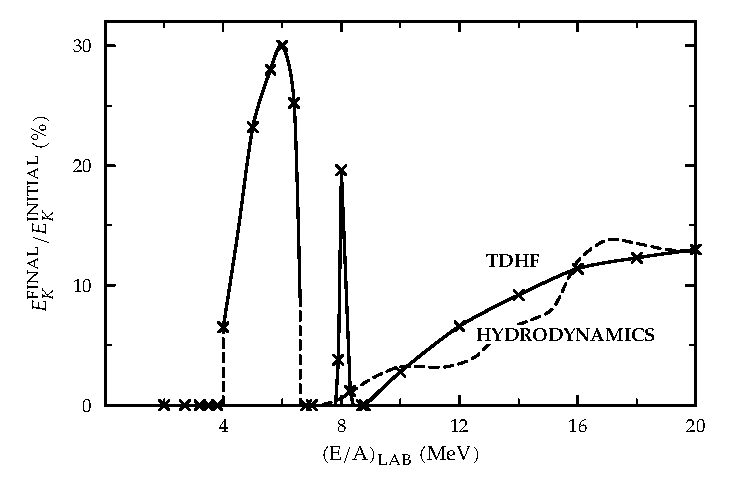
\includegraphics[width=0.8\textwidth]{pictures/12_4}
\par\end{centering}
\caption{\label{fig:12.4}两个核物质厚板碰撞中，末态平动动能与初态平动动能之比随 $E/A$ 的变化。零值表示聚变。（引自
\cite{BKN76}）虚线对应于 13.3.3 节中所讨论的流体力学计算。（引自 \cite{WMW77}）}
\end{figure}

厚板几何模型并不十分贴近现实，因为在 $x$ 和 $y$ 方向上的平移不变性阻止了核物质在碰撞过程中向侧面飞溅，并且高度的对称性削弱了阻尼机制。因此，二维
\cite{Ko76,CM76,MC76}、准三维 \cite{KDM77,MDK77} 以及全三维 \cite{CSM76,CMM78,BGK78,FW78}
计算相继被开展。这些计算需要耗费巨大的数值工作量，并给出了此类重离子散射过程中密度和流分布的清晰图像\footnote{关于重离子碰撞的导论，参见 \cite{NW76b}。}（见\ref{fig:12.5}）。

\begin{figure}[H]
\begin{centering}
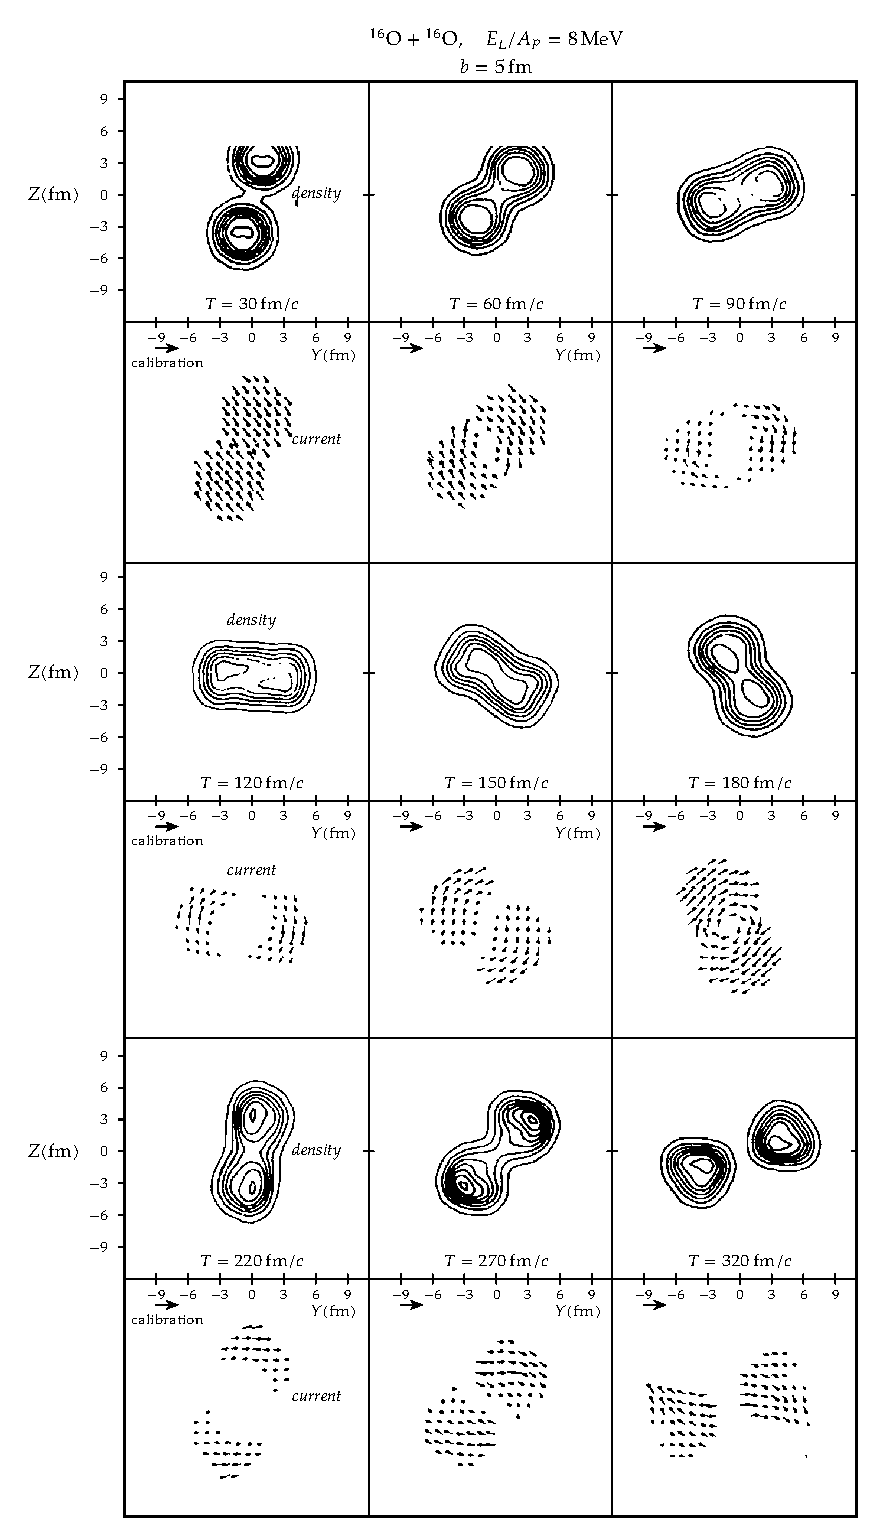
\includegraphics[width=0.85\textwidth]{pictures/12_5}
\par\end{centering}
\caption{\label{fig:12.5}在实验室参考系中，碰撞参数 $b=5\,\mathrm{fm}$ 时不同时刻 $T$ 下 $^{16}\mathrm{O}+{}^{16}\mathrm{O}$
碰撞的密度与速度分布。（引自 \cite{CMM78}）}
\end{figure}

TDHF 计算也被用于描述裂变过程 \cite{NKM78}。从极其接近鞍点处出发，系统演化一直被追踪至断裂为两个分离的碎片。然而在此我们不想进一步深入讨论利用
TDHF 理论所开展的大量数值计算细节。

\section{绝热时间相关Hartree-Fock理论（ATDHF）\label{sec:12.3}}

\subsection{ATDHF方程\label{subsec:12.3.1}}

正如我们在上一节所见，如今在某些情形下完全数值求解完整的 TDHF 方程是可能的。然而，对计算结果的解释却是困难的。因此，在本节中我们将研究一种作了进一步简化近似的理论：除了假定波函数在所有时刻都保持为
Slater 行列式（这构成了 TDHF 方法的特征）之外，我们仅考察缓慢过程并假设运动的速度很小。这一概念由 Belyaev \cite{Be65}
最早提出。其目标并非仅在于以某种近似求解 TDHF 方程 \ref{eq:12.9}，而是从中导出一个用于描述集体运动的 Bohr
型 Hamilton 量。正如我们将在 12.3.5.2 节所讨论的，对于诸如非简谐四极振动和低能重离子碰撞等多种集体运动，这一假设都是合理的；即使对于巨共振，绝热近似也是惊人地好的近似。

绝热近似有多种不同表述方式。最早的版本是由 Baranger 和 Kumar \cite{BK68} 在配对加四极力模型中引入的。后来，Baranger
和 Veneroni \cite{BV78}、Villars \cite{Vi75,Vi77}、Brink 等人 \cite{BEG76}
以及 Goeke 和 Reinhard \cite{GR78,RG78} 研究了更一般的形式体系。在这里，我们主要遵循 Baranger
和 Veneroni \cite{BV78} 的表述，因为在其中该理论的基本结构最为清晰；Villars 的方法将在 12.3.4
节中作更详细的探讨。结果表明，我们可以定义经典的坐标与正则共轭动量，它们服从经典的运动方程。

因此，首要问题在于定义这些坐标与动量。在 TDHF 理论中，一切均由单粒子密度 $\rho(t)$ 决定，而它在时间反演下并不是不变的。由于我们希望拥有时间反演不变的坐标，Baranger
和 Veneroni 提出了密度 $\rho(t)$ 的如下分解：

\begin{equation}
\rho(t)=\mathrm{e}^{\mathrm{i}\chi(t)/\hbar}\rho_{0}(t)\mathrm{e}^{-\mathrm{i}\chi(t)/\hbar}\label{eq:12.63}
\end{equation}

其中 $\rho_{0}$ 和 $\chi$ 都是 Hermitian 且在时间反演下为偶的矩阵，即：

\begin{equation}
\rho^{\dagger}_{0}=\rho_{0},\quad T\rho_{0}T^{-1}=\rho_{0};\qquad\chi^{\dagger}=\chi,\quad T\chi T^{-1}=\chi\label{eq:12.64}
\end{equation}

同样地，$\rho_{0}$ 满足 $\rho^{2}_{0}=\rho_{0}$，$\mathrm{Tr}\rho_{0}=N$，也就是说，它对应于一个
$N$ 维的 Slater 行列式 $|\Phi_{0}\rangle$。在下文中，$\rho_{0}$ 将作为坐标，并且正如我们将看到的，$\chi$
将作为动量。

相比于混合了时间反演偶分量与奇分量的 TDHF 密度 $\rho$，我们对以时间偶的行列式 $\rho_{0}$ 作为坐标要熟悉得多。例如在第
2 章中，我们使用了带有确定形变坐标 $q_{i}$ 的 Nilsson 函数，它们对应于时间偶的密度。对于带有时间偶约束的 CHF
计算（见 7.6 节），情况也是如此。

由 $\rho_{0}(t)$ 是时间偶的性质可得，与密度 $\rho_{0}(t)$ 相联系的总流密度在所有时刻均消失：

\begin{equation}
\boldsymbol{j}_{0}(\boldsymbol{r})=\mathrm{Tr}(\boldsymbol{j}\rho_{0})=0\label{eq:12.65}
\end{equation}

因为一个时间偶算符与一个时间奇算符乘积的迹必定为零，除非它是纯虚数。

因此在下文中，我们将 $\rho_{0}(t)$ 称为静态密度。它不应与与时间无关的密度相混淆，也不应与作为静态 HF 方程 $[h(\rho),\rho]=0$
之解的定态密度相混淆。然而结果表明，$\rho_{0}$ 是带有合适的（时间相关的）时间反演不变约束的静态 HF 方程的解 {[}见\ref{eq:12.120b}{]}。类似地，我们可以将
$\rho_{0}(t)$ 表示为：

\begin{equation}
\rho_{0}(t)=\mathrm{e}^{-\mathrm{i}\phi(t)/\hbar}\tilde{\rho}\mathrm{e}^{\mathrm{i}\phi(t)/\hbar}\label{eq:12.66}
\end{equation}

其中 $\phi(t)$ 是一个 Hermitian 时间奇算符，而 $\tilde{\rho}$ 是未受约束的静态 HF 问题
$[h(\tilde{\rho}),\tilde{\rho}]=0$ 的解。

在平移的情形下 {[}\ref{eq:12.32}{]}，我们已经见过密度 $\rho(t)$ 此类分解的一个范例，其中 $\chi$
为时间偶算符 $m\boldsymbol{v}\cdot\boldsymbol{r}$，而 $\phi$ 为时间奇算符 $t\boldsymbol{v}\cdot\boldsymbol{p}$。在转动的情形下
{[}\ref{eq:12.37}{]}，$(\boldsymbol{\omega}\cdot\boldsymbol{j})t$
是时间奇的，即它对应于算符 $\phi$。密度 $\tilde{\rho}$ 本身包含时间奇分量（见 7.7 节）且与时间无关。由于在此时不存在质心“角度”，在此情形下我们无法给出算符
$\chi$ 的显式表达式。\footnote{例如在 RPA 阶下，它已被计算为 Thouless-Valatin 方程 (8.106) 的解 $\Theta$。}

在下文中，我们将仅使用分解\ref{eq:12.63}。可以证明（见附录 D.2 节），在如下条件下该分解是唯一的：

(i) $\chi$ 的全部本征值 $\chi_{i}$ 满足：

\begin{equation}
-\frac{\pi\hbar}{2}<\chi_{i}\leqslant\frac{\pi\hbar}{2}\label{eq:12.67a}
\end{equation}

(ii) 在 $\rho_{0}$ 呈对角形式的基底中，$\chi$ 的 pp 和 hh 矩阵元消失，即：

\begin{equation}
\chi^{hh}=\rho_{0}\chi\rho_{0}=0;\qquad\chi^{pp}=\sigma_{0}\chi\sigma_{0}=0\label{eq:12.67b}
\end{equation}

这里我们利用了如下事实：在 $\rho_{0}$ 对角化的基底下，$\rho_{0}$ 是空穴态上的投影算符，而 $\sigma_{0}=1-\rho_{0}$
是粒子态上的投影算符。在下文中，我们将始终在该基底中展开。然而应当注意，由于 $\rho_{0}(t)$ 是时间的函数，该基底依赖于时间。

我们可能会问条件 \ref{eq:12.67a} 与 \ref{eq:12.67b} 是否是必要的。事实上并非如此；这仅仅是一个相当自然的选择，\footnote{然而已有研究表明，这一选择与假设 $\chi$ 在坐标空间中局域 \cite{BQ78} 是不相容的；有时局域的 $\chi$
似乎是自然的选择，正像我们在平移情形 {[}式 (12.32){]} 中所见的那样。}因为 pp 和 hh 矩阵元扮演着非常重要的角色。Baranger 和 Veneroni \cite{BV78} 已经证明，具有非零矩阵元
$\chi^{pp}$ 和 $\chi^{hh}$ 的任何其他分解所给出的结果，与我们在下文导出的结果之间的偏差，其阶数在 ATDHF
方法中本来就是被忽略的 $\chi$ 的高阶项。因此采用条件 \ref{eq:12.67a} 与 \ref{eq:12.67b}
与该近似是一致的，我们在下文中将采纳这些条件。

绝热近似现在体现为假设系统的密度 $\rho(t)$ 在所有时刻都接近于密度 $\rho_{0}(t)$，也就是说，我们在所有时刻都拥有一个近乎静态的密度。换言之，这意味着引入时间奇分量的矩阵
$\chi$ 是微小的。对于 TDHF 方程的所有解 $\rho(t)$ 而言这当然并不普遍成立，但我们仅仅对满足这一条件的解感兴趣。因此我们可以将
$\rho(t)$ 展开到 $\chi$ 的二阶：

\begin{equation}
\rho=\mathrm{e}^{\mathrm{i}\chi/\hbar}\rho_{0}\mathrm{e}^{-\mathrm{i}\chi/\hbar}\simeq\rho_{0}+\rho_{1}+\rho_{2}\label{eq:12.68}
\end{equation}

其中：

\begin{equation}
\rho_{1}=\frac{\mathrm{i}}{\hbar}[\chi,\rho_{0}],\qquad\chi=-\mathrm{i}\hbar[\rho_{1},\rho_{0}]\label{eq:12.69}
\end{equation}

\begin{equation}
\rho_{2}=-\frac{1}{2\hbar^{2}}[\chi,[\chi,\rho_{0}]]=\frac{1}{\hbar^{2}}\left(\chi\rho_{0}\chi-\frac{1}{2}(\chi^{2}\rho_{0}+\rho_{0}\chi^{2})\right)\label{eq:12.70}
\end{equation}

式 $(\text{D}.32)$ 表明 $\rho_{1}$ 仅具有 ph 和 hp 矩阵元，而 $\rho_{2}$ 仅具有
pp 和 hh 矩阵元：

\begin{equation}
\rho_{1}=\frac{\mathrm{i}}{\hbar}(\sigma_{0}\chi\rho_{0}-\rho_{0}\chi\sigma_{0})\label{eq:12.71}
\end{equation}

\begin{equation}
\rho_{2}=\frac{1}{\hbar^{2}}\left(\sigma_{0}\chi\rho_{0}\chi\sigma_{0}-\rho_{0}\chi\sigma_{0}\chi\rho_{0}\right)\label{eq:12.72}
\end{equation}

以完全相同的方式，我们可以展开\footnote{缩写符号 $\mathrm{Tr}_{1}$ 的定义见式 (E.19)。}：

\begin{equation}
h(\rho)=t+\mathrm{Tr}_{1}(\bar{v}\rho)=h_{0}+\Gamma_{1}+\Gamma_{2}\label{eq:12.73}
\end{equation}

其中：

\begin{equation}
h_{0}=t+\mathrm{Tr}_{1}(\bar{v}\rho_{0}),\qquad\Gamma_{1}=\mathrm{Tr}_{1}(\bar{v}\rho_{1}),\qquad\Gamma_{2}=\mathrm{Tr}_{1}(\bar{v}\rho_{2})\label{eq:12.74}
\end{equation}

在 $\rho$ 和 $h$ 的展开式中，偶数阶项在时间反演下总是偶的，而奇数阶项在时间反演下总是奇的。

如果我们将展开\ref{eq:12.68} 和 \ref{eq:12.73} 代入 TDHF 方程 \ref{eq:12.9}，我们可以根据它们在时间反演下的行为将其分解，从而得到两个
ATDHF 方程：

\begin{align}
(\mathrm{I})\qquad\mathrm{i}\hbar\dot{\rho}_{0} & =[h_{0},\rho_{1}]+[\Gamma_{1},\rho_{0}]\label{eq:12.75a}\\
(\mathrm{II})\qquad\mathrm{i}\hbar\dot{\rho}_{1} & =[h_{0},\rho_{0}]+[\Gamma_{1},\rho_{1}]+[\Gamma_{2},\rho_{0}]\label{eq:12.75b}
\end{align}

正如我们稍后将看到的，这两个方程仅有 ph 和 hp 部分是重要的。在导出这些方程时，我们忽略了 $\chi$ 的更高阶项。为了能够做到这一点，我们必须知道时间导数
$\dot{\rho}_{0},\dot{\rho}_{1},\dot{\rho}_{2}\dots$ 关于 $\chi$ 的阶数。在
Fourier 分析中，它们带有一个因子 $\omega$，其中 $\omega$ 为相应的频率。现在我们必须区分大振幅运动与小振幅振荡。在大振幅情形下，$\omega$
必须具有 $\chi$ 的数量级且微小；正如我们已经看到的，这意味着 $\dot{\rho}_{i}$ 比 $\rho_{i}$
在 $\chi$ 上高出一阶。在小振幅情形下，$\omega$ 并不必然与 $\chi$ 具有相同阶数，即 $\dot{\rho}_{i}$
与 $\rho_{i}$ 在 $\chi$ 上具有相同阶数。

因此在上述方程 (I) 中，我们略去了所有等于或高于二阶的项；在方程 (II) 中，我们略去了所有等于或高于三阶的项。此外，在方程
(II) 中略去了 $[h_{0},\rho_{2}]$ 项，其原因我们稍后将讨论。

在 $\chi$ 的零阶下，我们得到静态情形：

\begin{equation}
\dot{\rho}_{0}=0,\qquad[h_{0},\rho_{0}]=0\label{eq:12.76}
\end{equation}

因此方程 (I) 和 (II) 始终计入了关于 $\chi$ 的第一个非平凡阶次。特别地，这表明在大振幅情形下（其中 $\dot{\rho}_{1}$
为 $\chi$ 的二阶量），\ref{eq:12.75b} 中的 $[h_{0},\rho_{0}]$ 项也至少为二阶量，尽管
$h_{0}$ 与 $\rho_{0}$ 各自单独来看都是很大的量。这意味着静态 HF 方程 \ref{eq:12.76} 几乎被满足。原子核在所有时刻都几乎处于静态平衡状态，且运动是缓慢的。

正如我们将在 12.3.2 节中详细看到的，我们可以对 ATDHF 方程赋予经典诠释，其中 $\rho_{0}$ 和 $\chi$
是正则共轭的坐标和动量。方程 (I) 给出了速度 $\dot{\rho}_{0}$ 与动量 $\chi$ 之间的线性联系。相应的质量张量取决于坐标
$\rho_{0}$ 并依赖于时间。方程 (II) 在左端具有动量的时间导数。因此右端代表一个力。它依赖于 $[h_{0},\rho_{0}]$
项以及动量 $\chi$ 的二次项。从零速度下的某个初始值 $\rho_{0}$ 出发，$[h_{0},\rho_{0}]$
因此是在初始时刻加速系统的力。由于动量在所有时刻保持微小，$[h_{0},\rho_{0}]$ 在所有时刻的微小性因而是绝热运动存在的一个充要条件。如果在时间偶密度
$\rho_{0}$ 的空间中存在一个 $[h_{0},\rho_{0}]$ 微小的完整区域，那么我们便可以在该区域内找到一条对应于绝热运动的轨迹
$\rho(t)$。

我们仍须说明方程 (I) 和 (II) 应当仅在 ph 和 hp 空间中使用：方程 (I) 的 pp 和 hh 矩阵元至少为 $\chi$
的二阶量。例如，由式 $(\text{D}.32)$ 可知 $\dot{\rho}_{0}$ 仅具有 ph 和 hp 矩阵元，且由\ref{eq:12.71}
可知对 $\rho_{1}$ 也是如此。因此方程 (I) 右端的唯一非零 hh 矩阵元为：

\begin{equation}
\rho_{0}[h_{0},\rho_{1}]\rho_{0}=-\rho_{0}\left([h_{0},\rho_{0}]\rho_{1}+\rho_{1}[h_{0},\rho_{0}]\right)\rho_{0}\label{eq:12.77}
\end{equation}

它至少为二阶量，因为在大振幅情形下 $[h_{0},\rho_{0}]$ 为二阶量，而在小振幅情形下为一阶量。对于方程 (I) 的
pp 矩阵元，结论同样成立。

在方程 (II) 中，我们略去了 $[h_{0},\rho_{2}]$ 项。由\ref{eq:12.72} 可见，$\rho_{2}$
仅具有 hh 和 pp 矩阵元。因此 $[h_{0},\rho_{2}]$ 的 ph 矩阵元仅包含 $h_{0}$ 的 ph 和
hp 矩阵元，它们关于 $\chi$ 至少为一阶量。所以，在方程 (II) 的 hp 和 ph 部分中 $[h_{0},\rho_{2}]$
可以被忽略。在方程 (II) 的 hh 和 pp 部分中我们不能再忽略该项，因为 $h_{0}$ 的 pp 和 hh 矩阵元很大。然而我们可以证明，计入了
$[h_{0},\rho_{2}]$ 项的方程 (II) 的 pp 和 hh 矩阵元恒等于零。这需要较长的推导 \cite{BV78}；在此我们仅给出最重要的步骤。首先我们由\ref{eq:12.72}
表示 $\rho_{2}$；然后利用\ref{eq:12.71} 并得到 $\dot{\rho}_{1}$ 的 hh 矩阵元：

\begin{equation}
\rho_{0}\dot{\rho}_{1}\rho_{0}=-\dot{\rho}_{0}\rho_{1}\rho_{0}+\rho_{0}\rho_{1}\dot{\rho}_{0}\label{eq:12.78}
\end{equation}

最后，代入方程 (I) 对 $\dot{\rho}_{0}$ 的表达式，我们发现方程 (II) 的 pp 和 hh 部分恒消失。

如果我们从某些初始值 $\rho_{0}(0),\rho_{1}(0)$ 或者 $\rho_{0}(0)$ 和 $\dot{\rho}_{0}(0)$
出发，ATDHF 方程组 \ref{eq:12.75a} 与 \ref{eq:12.75b} 允许我们在所有时刻计算 $\rho_{0}(t)$
和 $\rho_{1}(t)$。然而，这一问题的求解至少与精确 TDHF 方程一样困难，在实践中没有人会这样做。绝热理论的主要优势在于：它允许我们导出一个用于描述集体运动的经典
Hamilton 量。

\subsection{集体Hamilton量\label{subsec:12.3.2}}

我们现在能够用变量 $\rho_{0}$ 和 $\rho_{1}$（或 $\rho_{0}$ 和 $\chi$）来表达系统的总能量
$E$。由式 $(5.28)$，我们求得：

\begin{equation}
E=\mathrm{Tr}(t\rho)+\frac{1}{2}\mathrm{Tr}_{1}\mathrm{Tr}_{2}(\rho\bar{v}\rho)=\mathcal{K}+\mathcal{V}\label{eq:12.79}
\end{equation}

其中我们将所有依赖于速度二阶的项归入动能 $\mathcal{K}$ 中，并将所有仅包含静态密度 $\rho_{0}$ 的项归入势能
$\mathcal{V}$ 中。由于 Hamilton 量的时间反演不变性，关于 $\rho_{1}$ 的线性项消失。我们求得
$\mathcal{V}$ 为密度分布 $\rho_{0}$ 的静态 HF 能量：

\begin{equation}
\mathcal{V}=\mathrm{Tr}(t\rho_{0})+\frac{1}{2}\mathrm{Tr}_{1}\mathrm{Tr}_{2}(\rho_{0}\bar{v}\rho_{0})\label{eq:12.80}
\end{equation}

动能具有如下形式：

\begin{equation}
\mathcal{K}=\mathrm{Tr}(h_{0}\rho_{2})+\frac{1}{2}\mathrm{Tr}_{1}\mathrm{Tr}_{2}(\rho_{1}\bar{v}\rho_{1})\label{eq:12.81}
\end{equation}

它二次方地依赖于 $\rho_{1}$（或 $\chi$），并且由于\ref{eq:12.75a}，也二次方地依赖于速度 $\dot{\rho}_{0}$。我们可以用几种方式来书写它。首先，我们采用使得
$h_{0}$ 的 pp 部分与 hh 部分均对角化的基底。这总是可行的，因为 $\rho_{0}$ 在这种变换下保持不变。我们将本征值记为
$\epsilon_{m}$（粒子）和 $\epsilon_{i}$（空穴）。利用\ref{eq:12.69} 以及定义：

\begin{align}
A_{minj} & =(\epsilon_{m}-\epsilon_{i})\delta_{nm}\delta_{ij}+\bar{v}_{mjin}\nonumber \\
B_{minj} & =\bar{v}_{mnij}\label{eq:12.82}
\end{align}

利用 $\chi_{im}=\chi^{*}_{mi}$，我们求得：

\begin{equation}
\mathcal{K}=\frac{1}{2\hbar^{2}}(\chi^{*},\chi)\left(\begin{array}{cc}
A & B\\
B^{*} & A^{*}
\end{array}\right)\left(\begin{array}{c}
\chi\\
\chi^{*}
\end{array}\right)\label{eq:12.83}
\end{equation}

其中在 $(\chi_{mi},\chi^{*}_{mi})$ 中矩阵的指标遍历所有 ph 对 $(mi)$。它看起来与第 8
章中的 RPA 记号非常相似。然而它更为普遍，因为单粒子能量与 $\chi$ 都依赖于时间。

我们也可以在这种记号下书写 ATDHF 方程 (I)：

\begin{equation}
\hbar\left(\begin{array}{c}
\dot{\rho}_{0}\\
-\dot{\rho}^{*}_{0}
\end{array}\right)=\left(\begin{array}{cc}
A & B\\
B^{*} & A^{*}
\end{array}\right)\left(\begin{array}{c}
\chi\\
\chi^{*}
\end{array}\right)\label{eq:12.84}
\end{equation}

它联系了速度与动量，并表明矩阵：

\begin{equation}
\mathfrak{M}=\hbar^{2}\left(\begin{array}{cc}
A & B\\
B^{*} & A^{*}
\end{array}\right)^{-1}\label{eq:12.85}
\end{equation}

代表一个依赖于坐标 $\rho_{0}$ 的质量张量。容易看出，在转动情形下它对应于转动惯量的 Thouless-Valatin
值 $(8.142)$。动能\ref{eq:12.83} 具有形式：

\begin{equation}
\mathcal{K}=\frac{1}{2}(\dot{\rho}^{*}_{0},-\dot{\rho}_{0})\mathfrak{M}\left(\begin{array}{c}
\dot{\rho}_{0}\\
-\dot{\rho}^{*}_{0}
\end{array}\right)\label{eq:12.86}
\end{equation}

我们因此导出了一个经典的 Hamilton 函数，它依赖于坐标 $\rho_{0}$ 并二次方地依赖于动量 $\chi$：

\begin{equation}
\mathcal{H}(\chi,\rho_{0})=\frac{1}{2\hbar^{2}}(\chi^{*},\chi)\mathfrak{M}^{-1}\left(\begin{array}{c}
\chi\\
\chi^{*}
\end{array}\right)+\mathcal{V}(\rho_{0})\label{eq:12.87}
\end{equation}

$\mathcal{V}(\rho_{0})=\langle\Phi|H|\Phi\rangle$ 是完整 Hamilton 量在静态波函数
$|\Phi\rangle$ 下的期望值。动能完全源自波函数的时间奇分量。正如我们从\ref{eq:12.81} 所见，它由两项贡献组成。第一项包含静态势
$h_{0}$，第二项包含由于时间奇密度分量 $\rho_{1}$ 引起的自洽势重整化效应。如果我们略去自洽场的这一重整化效应（例如在唯象势中），质量张量
\ref{eq:12.85} 中的矩阵 $B$ 将消失，我们将获得 Inglis 公式（参见 8.4.7 节）。

为了使形式体系完备，我们必须说明可以从 Hamilton 变分原理得到 ATDHF 方程。对固定的 $\rho_{0}$，我们求得：

\begin{equation}
\frac{\partial\mathcal{H}}{\partial\chi^{*}}=\frac{1}{\hbar^{2}}\mathfrak{M}^{-1}\left(\begin{array}{c}
\chi\\
\chi^{*}
\end{array}\right)=\dot{\rho}_{0}\label{eq:12.88}
\end{equation}

这表明第一个 ATDHF 方程 {[}对应于\ref{eq:12.84}{]} 与 Hamilton 方程 $\dot{q}=\partial\mathcal{H}/\partial p$
完全等价。第二个 ATDHF 方程的推导更为复杂。我们首先计算由改变 $\delta\rho_{0}$ 所引起的 $\rho_{1}$
和 $\rho_{2}$ 的变化。对固定的 $\chi$，由\ref{eq:12.69} 和 \ref{eq:12.70}
可得：

\begin{equation}
\delta\rho_{1}=\frac{\mathrm{i}}{\hbar}[\chi,\delta\rho_{0}],\qquad\delta\rho_{2}=-\frac{1}{2\hbar^{2}}[\chi,[\chi,\delta\rho_{0}]]\label{eq:12.89}
\end{equation}

因此能量 \ref{eq:12.79} 的改变量为：

\begin{equation}
\delta E=\mathrm{Tr}(\Gamma_{2}\delta\rho_{0}+\Gamma_{1}\delta\rho_{1}+h_{0}\delta\rho_{2})+\delta\mathcal{V}\label{eq:12.90}
\end{equation}

由于 $\chi$ 和 $\delta\rho_{0}$ 仅有 ph 和 hp 矩阵元，$h_{0}$ 对这些迹有贡献的唯一矩阵元是
ph 和 hp 矩阵元。正如在上一小节中所讨论的，它们关于 $\chi$ 至少为一阶量。为了保持自洽，我们因此必须略去\ref{eq:12.90}
中的最后一项，并求得第二个 Hamilton 方程：

\begin{equation}
-\dot{\chi}=\frac{\partial\mathcal{H}}{\partial\rho_{0}}=\frac{\partial\mathcal{K}}{\partial\rho_{0}}+\frac{\partial\mathcal{V}}{\partial\rho_{0}}\label{eq:12.91}
\end{equation}

当然，我们只需使用这些方程的 ph 和 hp 矩阵元。结合：

\begin{equation}
\rho_{0}\dot{\rho}_{1}\rho_{0}=-\frac{\mathrm{i}}{\hbar}\dot{\chi}\label{eq:12.92}
\end{equation}

以及静态能量对密度 $\rho_{0}$ 的微商 $\partial\mathcal{V}/\partial\rho_{0}$
给出了 $h_{0}$ 的 ph 矩阵元 {[}见式 $(5.32)${]} 的事实，我们看到\ref{eq:12.91} 精确对应于第二个
ATDHF 方程 \ref{eq:12.75b}。

因此，第二个 ATDHF 方程描述了系统的加速度。除了静态力 $(\partial\mathcal{V}/\partial\rho_{0})$
之外，还存在源于质量张量 \ref{eq:12.85} 对坐标的依赖性的附加项。

利用 Hamilton 形式体系，我们现已建立了与经典系统的完全类比。我们也可以利用 Lagrange 形式体系来完成这一点 \cite{BV78}。

在小振幅极限下，我们可以用一种不同于通常方式（见 8.4 节）的方法导出 RPA。我们假设 $\rho_{0}(t)$ 保持接近于静态
HF 问题 $[h(\tilde{\rho}),\tilde{\rho}]=0$ 的定态解 $\tilde{\rho}$：

\begin{equation}
\rho_{0}(t)=\tilde{\rho}+\xi(t)\label{eq:12.93}
\end{equation}

并将势能 $\mathcal{V}(\rho_{0})$ 在点 $\tilde{\rho}$ 处展开至二阶 {[}见式 $(7.34)${]}：

\begin{equation}
\mathcal{V}(\rho_{0})=\mathcal{V}(\tilde{\rho})+\frac{1}{2}(\xi^{*},\xi)\mathfrak{S}\left(\begin{array}{c}
\xi\\
\xi^{*}
\end{array}\right)\label{eq:12.94}
\end{equation}

利用稳定性矩阵 $\mathfrak{S}$ {[}式 $(7.37)${]}（曲率张量），我们得到能量：

\begin{equation}
\mathcal{H}=\frac{1}{2\hbar^{2}}(\chi^{*},\chi)\mathfrak{M}^{-1}\left(\begin{array}{c}
\chi\\
\chi^{*}
\end{array}\right)+\frac{1}{2}(\xi^{*},\xi)\mathfrak{S}\left(\begin{array}{c}
\xi\\
\xi^{*}
\end{array}\right)\label{eq:12.95}
\end{equation}

这是耦合谐振子的 Hamilton 函数。相应的运动方程由频率为 $\Omega$ 的简谐振动求解，我们最终得到本征值问题 \cite{Go59}：

\begin{equation}
\mathfrak{M}\Omega^{2}\mathfrak{X}=\mathfrak{S}\mathfrak{X}\label{eq:12.96}
\end{equation}

频率 $(\hbar\Omega)$ 是矩阵：

\begin{equation}
\left(\begin{array}{cc}
A & B\\
-B^{*} & -A^{*}
\end{array}\right)=\sigma_{3}\mathfrak{M}^{-1},\qquad\sigma_{3}=\left(\begin{array}{cc}
1 & 0\\
0 & -1
\end{array}\right)\label{eq:12.97}
\end{equation}

的本征值。它们可以通过仅对 $\mathfrak{M}^{-1}\mathfrak{S}$ 进行对角化来求得，这正是 RPA 矩阵。这之所以可能，仅仅是因为质量张量
$\mathfrak{M}$ 的逆矩阵具有与曲率张量 $\mathfrak{S}$ 类似的结构。

\subsection{约化为少数集体坐标\label{subsec:12.3.3}}

我们回到大振幅问题。ATDHF 方程组 \ref{eq:12.75a} 与 \ref{eq:12.75b} 仍包含所有自由度，对于实际应用而言过于普遍。特别地，它并不比完整的
TDHF 方程 \ref{eq:12.9} 更易求解；然而，绝热近似也仅对少数轨道有效。因此，大幅度减少自由度的数目应当是可能的。

选择合适的集体变量当然是一个重大问题。在深入讨论此问题之前，我们首先假设已经实现了这种约化，并拥有一个时间偶的 Slater 行列式族：

\begin{equation}
|\Phi(\boldsymbol{q})\rangle=|\Phi(q_{1}\dots q_{f})\rangle\label{eq:12.98}
\end{equation}

以及相应的密度 $\rho_{0}(\boldsymbol{q})$，它们具有如下性质：ATDHF 问题的解将始终保持在由实参数
$\boldsymbol{q}$ 所表征的该 Slater 行列式子集之内；即存在一条路径 $\boldsymbol{q}(t)$
满足：

\begin{equation}
\rho_{0}(t)=\rho_{0}(\boldsymbol{q}(t))\label{eq:12.99}
\end{equation}

由此我们求得速度：

\begin{equation}
\dot{\rho}_{0}=\sum^{f}_{\mu=1}\dot{q}_{\mu}\frac{\partial\rho_{0}}{\partial q_{\mu}}\label{eq:12.100}
\end{equation}

正如在附录 D.3 节中所展示的，Hermitian 矩阵 $\partial\rho_{0}/\partial q_{\mu}$
在 $\rho_{0}$ 为对角的基底下仅具有 ph 和 hp 矩阵元，且等于厄米单粒子算符 $\hat{\boldsymbol{P}}=(\hat{P}_{1},\dots,\hat{P}_{f})$
的相应矩阵元\footnote{这些矩阵对应于式 (12.32) 中的矩阵 $p$。我们在此使用大写字母 $P$ 以区别于集体动量 $p$ {[}式 (12.104){]}。}。单粒子矩阵
$\boldsymbol{P}$ 具有矩阵元 {[}见式 (D.36) 及以下{]}：

\begin{equation}
\boldsymbol{P}_{mi}=\boldsymbol{P}^{*}_{im}=-\langle m|\frac{\hbar}{\mathrm{i}}\frac{\partial}{\partial\boldsymbol{q}}|i\rangle;\qquad\boldsymbol{P}_{mm^{\prime}}=\boldsymbol{P}_{ii^{\prime}}=0\label{eq:12.101}
\end{equation}

在 $\rho_{0}$ 对角化的基底下。

既然我们现在有了速度 $\dot{\rho}_{0}$ 关于 $\dot{\boldsymbol{q}}$ 的显式表达式，由\ref{eq:12.86}
和 \ref{eq:12.100}，我们得到动能：

\begin{equation}
\mathcal{K}=\frac{1}{2}\sum^{f}_{\mu,\mu^{\prime}=1}M_{\mu\mu^{\prime}}(\boldsymbol{q})\dot{q}_{\mu}\dot{q}_{\mu^{\prime}}\label{eq:12.102}
\end{equation}

以及实的集体质量张量：

\begin{equation}
M_{\mu\mu^{\prime}}(\boldsymbol{q})=\frac{1}{\hbar^{2}}(P^{*}-P)_{\mu}\mathfrak{M}\left(\begin{array}{c}
P\\
-P^{*}
\end{array}\right)_{\mu^{\prime}}\label{eq:12.103}
\end{equation}

我们还可以定义集体动量 $p_{\mu}$，并由\ref{eq:12.84} 和 \ref{eq:12.100} 求得：

\begin{equation}
p_{\mu}=\sum_{\mu^{\prime}}M_{\mu\mu^{\prime}}(\boldsymbol{q})\dot{q}_{\mu^{\prime}}=\mathrm{Tr}\left(\chi\frac{\partial\rho_{0}}{\partial q_{\mu}}\right)=\mathrm{Tr}\left(\chi\frac{\partial}{\partial q_{\mu}}\rho_{0}\right)\label{eq:12.104}
\end{equation}

能量呈现出经典 Hamilton 函数的形式：

\begin{equation}
\mathcal{H}(\boldsymbol{p},\boldsymbol{q})=\frac{1}{2}\sum_{\mu\mu^{\prime}}M^{-1}_{\mu\mu^{\prime}}(\boldsymbol{q})p_{\mu}p_{\mu^{\prime}}+\mathcal{V}(\boldsymbol{q})\label{eq:12.105}
\end{equation}

为了证明我们真正拥有一个正则系统，我们必须验证从函数 \ref{eq:12.105} 导出的 Hamilton 方程。第一个方程由下式直接给出：

\begin{equation}
\frac{\partial\mathcal{H}}{\partial p_{\mu}}=\sum_{\mu^{\prime}}M^{-1}_{\mu\mu^{\prime}}p_{\mu^{\prime}}=\dot{q}_{\mu}\label{eq:12.106}
\end{equation}

在第二个方程的情形下，利用\ref{eq:12.87}、\ref{eq:12.90} 和 \ref{eq:12.104}，并在一种显然的简记符号
\cite{BGV76} 下，我们得到：

\begin{align}
\frac{\partial\mathcal{H}}{\partial q_{\mu}} & =\frac{\partial E}{\partial\rho^{*}_{0}}\frac{\partial\rho_{0}}{\partial q_{\mu}}+\frac{\partial E}{\partial\chi^{*}}\frac{\partial\chi}{\partial q_{\mu}}=-\dot{\chi}\frac{\partial\rho_{0}}{\partial q_{\mu}}+\dot{\rho}_{0}\frac{\partial\chi}{\partial q_{\mu}}\nonumber \\
 & =-\dot{\chi}\frac{\partial\rho_{0}}{\partial q_{\mu}}-\chi\frac{\mathrm{d}}{\mathrm{d}t}\frac{\partial\rho_{0}}{\partial q_{\mu}}+\sum_{\mu^{\prime}}\dot{q}_{\mu^{\prime}}\frac{\partial}{\partial q_{\mu}}\left(\chi\frac{\partial}{\partial q_{\mu^{\prime}}}\rho_{0}\right)\nonumber \\
 & =-\frac{\mathrm{d}}{\mathrm{d}t}\left(\chi\frac{\partial\rho_{0}}{\partial q_{\mu}}\right)+\sum_{\mu^{\prime}}\dot{q}_{\mu^{\prime}}\frac{\partial}{\partial q_{\mu}}p_{\mu^{\prime}}\nonumber \\
 & =-\frac{\mathrm{d}}{\mathrm{d}t}p_{\mu}\label{eq:12.107}
\end{align}

因为 $p_{\mu}$ 和 $q_{\mu}$ 是独立变量 $[(\partial/\partial q_{\mu})p_{\mu^{\prime}}=0]$。

人们还经常引入一组仅具有 ph 和 hp 矩阵元的 Hermitian 算符 $\hat{\boldsymbol{Q}}$，其定义为：

\begin{equation}
\left(\begin{array}{c}
Q\\
Q^{*}
\end{array}\right)_{\mu}=\frac{\hbar}{\mathrm{i}}\sum_{\mu^{\prime}}M^{-1}_{\mu\mu^{\prime}}\left(\begin{array}{cc}
A & -B\\
-B^{*} & A^{*}
\end{array}\right)^{-1}\left(\begin{array}{c}
P\\
-P^{*}
\end{array}\right)_{\mu^{\prime}}\label{eq:12.108}
\end{equation}

它们与算符 $\chi$ 密切相关：

\begin{equation}
\chi=\sum_{\mu}p_{\mu}Q_{\mu}\label{eq:12.109}
\end{equation}

质量张量 \ref{eq:12.103} 也可以表示为：

\begin{equation}
M_{\mu\mu^{\prime}}(\boldsymbol{q})=(Q^{*},Q)_{\mu}\left(\begin{array}{cc}
A & B\\
B^{*} & A^{*}
\end{array}\right)\left(\begin{array}{c}
Q\\
Q^{*}
\end{array}\right)_{\mu^{\prime}}\label{eq:12.110}
\end{equation}

算符 $\hat{\boldsymbol{P}}$ 和 $\hat{\boldsymbol{Q}}$ 服从归一化条件：

\begin{equation}
\langle\Phi_{0}|[\hat{P}_{\mu},\hat{Q}_{\mu^{\prime}}]|\Phi_{0}\rangle=\mathrm{Tr}(\rho_{0}[P_{\mu},Q_{\mu^{\prime}}])=\frac{\hbar}{\mathrm{i}}\delta_{\mu\mu^{\prime}}\label{eq:12.111}
\end{equation}

由于 $\boldsymbol{P}$ 仅具有 ph 和 hp 矩阵元，算符 $\hat{\boldsymbol{P}}$ 由\ref{eq:12.101}
唯一确定。它完全由静态波函数族 $|\Phi_{0}(\boldsymbol{q})\rangle$ 所给出。如果我们已知“动量”
$\boldsymbol{p}$ {[}\ref{eq:12.104}{]} 以及“坐标” $\boldsymbol{q}$，我们便获得时间相关的
Slater 行列式：

\begin{equation}
|\Phi(\boldsymbol{p},\boldsymbol{q})\rangle=\mathrm{e}^{\mathrm{i}\sum_{\mu}p_{\mu}\hat{Q}_{\mu}/\hbar}|\Phi_{0}(\boldsymbol{q})\rangle\label{eq:12.112}
\end{equation}

如果我们将动量 $\boldsymbol{p}$ 视为一个微分算符 $(\hbar/\mathrm{i})\partial/\partial\boldsymbol{q}$，这在某种意义上看起来像一个
Taylor 展开，但事实并非如此，因为 $\hat{\boldsymbol{Q}}$ 依赖于 $\boldsymbol{q}$，且
$\hat{\boldsymbol{Q}}$ 与 $\hat{\boldsymbol{P}}$ 并不对易。只有在微小 $\boldsymbol{p}$
的极限下，由\ref{eq:12.111} 我们才能导出：

\begin{equation}
|\Phi(\boldsymbol{p},\boldsymbol{q})\rangle\simeq\left(1+\sum_{\mu}p_{\mu}\frac{\partial}{\partial p_{\mu}}\right)|\Phi(\boldsymbol{p}=0,\boldsymbol{q})\rangle\label{eq:12.113}
\end{equation}

该理论的一个范例（其中 $\hat{\boldsymbol{P}}$ 和 $\hat{\boldsymbol{Q}}$ 是精确的常数算符）由
Galilei 变换给出 {[}见\ref{eq:12.32}{]}。

\subsection{集体坐标的选取\label{subsec:12.3.4}}

在导出 Hamilton 量 \ref{eq:12.105} 时，我们假设我们已经能够找到一个静态行列式族 $|\Phi_{0}(\boldsymbol{q})\rangle$，具有如下性质：在某些初始条件下
ATDHF 方程 \ref{eq:12.75a} 与 \ref{eq:12.75b} 的解对应于贯穿该子集的一条轨道。在一般情形下，此类子集将仅包含单一的一维轨道。然而在某些情况下，也可以找到高维超曲面，使得
ATDHF 问题 \ref{eq:12.75a} 与 \ref{eq:12.75b} 的解对于许多不同的初始条件均保持在该子集之内。例如，这在转动情形下是显然成立的，此时超曲面由
Euler 角所参数化。

在导出集体 Hamilton 量 \ref{eq:12.105} 时，我们假设我们已经选定了该子集 $\rho_{0}(\boldsymbol{q})$。然后，我们仅使用了第一个
ATDHF 方程 \ref{eq:12.75a} 来计算相应的动量与惯性参数。第二个方程 \ref{eq:12.75b} 仅被用于导出经典运动方程
\ref{eq:12.107}。我们根本没有考察它是否被给定的路径 $\rho_{0}(\boldsymbol{q})$ 所满足。事实上，在一般情形下它并不会被满足。在
12.3.1 节中我们看到，为了满足第二个 ATDHF 方程，我们至少必须要求：

\begin{equation}
[h_{0}(\rho_{0}),\rho_{0}]=\mathcal{O}(\chi^{2})\label{eq:12.114}
\end{equation}

这并不是对所有路径都自动成立的。如果我们在 $\rho_{0}$ 的空间中任意选取一条路径，沿着该路径计算质量参数与势能并求解经典运动方程
\ref{eq:12.106} 和 \ref{eq:12.107}，那么该解一般而言并不构成 ATDHF 方程 \ref{eq:12.75a}
与 \ref{eq:12.75b} 的解。Villars \cite{Vi75,Vi77} 利用第二个方程来确定最优路径 $\rho_{0}(q)$。为简便起见，我们在下文中局限于单一集体坐标
$q$。

正如我们在 12.3.1 节所指出的，该方程仅有 ph 和 hp 部分是有意义的。利用\ref{eq:12.69}，它可以写为：

\begin{equation}
\dot{\chi}=-[h_{0},\rho_{0}]-[\Gamma_{1},\rho_{1}]-[\Gamma_{2},\rho_{0}]\label{eq:12.115}
\end{equation}

由于 $[h_{0},\rho_{0}]$ 具有时间偶性且仅有 ph 和 hp 矩阵元，我们可以将其写为某个时间偶 Hermitian
单粒子算符 $F$ 与 $\rho_{0}$ 的对易子：

\begin{equation}
[h_{0},\rho_{0}]=[F,\rho_{0}]\label{eq:12.116}
\end{equation}

我们假设已知第一个 ATDHF 方程的解 $\chi$ 并使用\ref{eq:12.109}。$\chi$ 的时间导数随后由下式给出：

\begin{equation}
\dot{\chi}=MQ\ddot{q}+\dot{q}^{2}\frac{\mathrm{d}}{\mathrm{d}q}(MQ)\label{eq:12.117}
\end{equation}

结合运动方程 \ref{eq:12.106} 和 \ref{eq:12.107}，我们求得：

\begin{equation}
\ddot{q}=\frac{\mathrm{d}}{\mathrm{d}t}\frac{p}{M}=-\frac{1}{M}\frac{\mathrm{d}\mathcal{V}}{\mathrm{d}q}-\frac{\dot{q}^{2}}{2}\frac{1}{M}\frac{\mathrm{d}M}{\mathrm{d}q}\label{eq:12.118}
\end{equation}

由于 $\Gamma_{2}$ 和 $[\Gamma_{1},\chi]$ 关于 $\dot{q}$ 是二次的，利用\ref{eq:12.116}，对于约束算符
$F$ 我们求得：

\begin{equation}
F=\frac{\mathrm{d}\mathcal{V}}{\mathrm{d}q}\cdot Q+\mathcal{O}(\dot{q}^{2})\label{eq:12.119}
\end{equation}

为了获得自洽的描述，正比于 $\dot{q}^{2}$ 的项必须微小并被略去。我们因此得到从受约束 HF 方程确定路径 $\rho_{0}(q)$
的可能性，其中约束 $Q$ 由\ref{eq:12.108} 给出。该方程中的质量参数 $M(q)$ 例如可由条件 \ref{eq:12.111}
确定。如下一组方程（Villars 方程 \cite{Vi75,Vi77}）在略去 $\dot{q}^{2}$ 阶项的意义下等价于
ATDHF 方程 \ref{eq:12.75a} 与 \ref{eq:12.75b}：

\begin{align}
\left(\begin{array}{cc}
A & -B\\
-B^{*} & A^{*}
\end{array}\right)\left(\begin{array}{c}
Q\\
Q^{*}
\end{array}\right) & =\frac{\hbar}{\mathrm{i}M}\left(\begin{array}{c}
P\\
-P^{*}
\end{array}\right)\label{eq:12.120a}\\
\left[h_{0}-\frac{\mathrm{d}\mathcal{V}}{\mathrm{d}q}Q,\rho_{0}\right] & =0\label{eq:12.120b}\\
\langle\Phi_{0}|[\hat{P},\hat{Q}]|\Phi_{0}\rangle & =\frac{\hbar}{\mathrm{i}}\label{eq:12.120c}
\end{align}

该系统与我们在生成坐标法中通过自洽确定路径所得到的系统极为相似（见 10.8 节）。对于实际应用，我们必须从对\ref{eq:12.120b}
中约束算符的某个初始猜测出发，并计算相应的 $\rho_{0}(q)$。由\ref{eq:12.100}，我们可以在每个点 $q$
处确定相应的算符 $P$，并从\ref{eq:12.120a} 确定一个新的约束算符 $Q$。这一过程必须迭代进行，直至实现收敛。

与此有某种联系的是局域简谐近似（local harmonic approach）\cite{HY74,RB76,Ma77b,ABC77b,MV77}，其中
$P$ 在线性响应近似下由\ref{eq:12.120b} 确定 {[}见式 $(8.137)${]}，略去曲率修正 \cite{RG77}：

\begin{equation}
\left(\begin{array}{cc}
A & -B\\
-B^{*} & A^{*}
\end{array}\right)\left(\begin{array}{c}
P\\
P^{*}
\end{array}\right)=\mathrm{i}\hbar C\left(\begin{array}{c}
Q\\
-Q^{*}
\end{array}\right)\label{eq:12.121}
\end{equation}

其中 $C=(\mathrm{d}^{2}\mathcal{V}/\mathrm{d}q^{2})$，即势能的曲率。然后我们可以定义集体频率
$\Omega(q)$ \cite{RB76}：

\begin{equation}
\Omega(q)=\sqrt{\frac{C(q)}{M(q)}}\label{eq:12.122}
\end{equation}

以及玻色子算符：

\begin{equation}
A^{\dagger}(q)=\sqrt{\frac{M\Omega}{2\hbar}}\left(\hat{Q}-\mathrm{i}\frac{1}{M\Omega}\hat{P}\right)\label{eq:12.123}
\end{equation}

由于\ref{eq:12.120a} 和 \ref{eq:12.121} 精确对应于形式为 $(8.99)$ 的 RPA 方程，算符
$A^{\dagger}$ 可以作为在每个点 $q$ 处进行 RPA 计算（局域 RPA）的解求得。

在此我们不想进一步深入这些及类似方法的细节，这些方法目前仍在积极研究中。总结本小节的结果，我们可以说：存在着在所有 Slater 行列式的广大集合中确定一条最优路径或一个最优超曲面（在我们需要多于一个集体坐标的情形下）的方法。我们从而获得了能量表达\ref{eq:12.105}，即经典的
Hamilton 函数。

\subsection{ATDHF方法的一般讨论\label{subsec:12.3.5}}

\subsubsection{为什么需要重新量子化？}

ATDHF 方法最终导出一个经典的运动方程。系统的激发能和波函数可以通过求解经典运动方程 \ref{eq:12.106} 和 \ref{eq:12.107}
来获得。在量子力学情形下，我们必须首先重新量子化该经典 Hamilton 量（如 1.5 节所讨论的）。这一处方并非像乍看起来那样完全是唯象的，因为可以证明
\cite{MH72,BM78}，通过将精确玻色展开（见第 9 章）中的玻色子算符或相应的动量与坐标算符替换为 $c$ 数，可以得到完整的
TDHF 理论。在这个意义上，TDHF 以及 ATDHF 都是经典理论，因此对其进行重新量子化似乎是自然的。然而，这并不意味着该理论是完全经典的；归根结底，Slater
行列式是一个量子力学波函数。

我们已经在 12.2.4 节中看到，将波函数限制为 Slater 行列式包含着某些经典特征，诸如无弥散的孤子解。如果我们将自己限制在少数几个集体变量
$\boldsymbol{q}$ 上，这些特征甚至更加显著。如果 $\boldsymbol{q}$ 是一个集体变量，两个波函数
$|\Phi(\boldsymbol{q})\rangle$ 和 $|\Phi(\boldsymbol{q}^{\prime})\rangle$
之间的重叠在 $\boldsymbol{q}=\boldsymbol{q}^{\prime}$ 处表现出极为尖锐的极大（见 10.7.4
节），即在很好的近似下我们可以写为：

\begin{equation}
\langle\Phi(\boldsymbol{q})|\Phi(\boldsymbol{q}^{\prime})\rangle\simeq\delta(\boldsymbol{q}-\boldsymbol{q}^{\prime})\label{eq:12.124}
\end{equation}

这表明函数 $|\Phi(\boldsymbol{q})\rangle$ 是在 $q$ 空间中高度局域化的波包。与此同时，我们计算了
$\dot{\boldsymbol{q}}$，这违背了测不准关系，因而是经典近似。在完全的量子力学理论中，我们应当使用许多不同形状
$|\Phi(\boldsymbol{q})\rangle$ 的叠加，正如我们在 GCM 方法（见第 10 章）中所做的那样。

\subsubsection{绝热近似的有效性}

我们现在能够给出绝热近似成立的粗略判据 \cite{BV78}。为此，我们限制讨论单一集体变量 $q$（这事实上并非限制，因为
$q$ 可以是 ATDHF 方程的精确解）。

绝热方法等价于要求任何单粒子波函数中的时间奇分量：

\begin{equation}
\mathrm{e}^{\mathrm{i}\hat{\chi}}|i\rangle\simeq|i\rangle+\mathrm{i}\hat{\chi}|i\rangle\label{eq:12.125}
\end{equation}

应具有很小的模长：

\begin{equation}
|\hat{\chi}|i\rangle|^{2}=\sum_{m}|\langle m|\hat{\chi}|i\rangle|^{2}\ll1\qquad\text{对所有 }i\text{ 成立。}\label{eq:12.125b}
\end{equation}

作为粗略估计，如果我们在\ref{eq:12.83} 中略去剩余相互作用——即如果我们使用集体质量的 Inglis 公式——我们求得参与该运动的动能为：

\begin{equation}
\mathcal{K}=\sum_{mi}\chi^{*}_{mi}(\epsilon_{m}-\epsilon_{i})\chi_{mi}\simeq\Delta\epsilon\sum_{mi}|\chi_{mi}|^{2}\label{eq:12.126}
\end{equation}

其中 $\Delta\epsilon$ 为典型的 ph 能量。如果我们进一步假设时间奇分量的掺杂均匀分布在 $N$ 个占据态上，由\ref{eq:12.126}
我们得到绝热性条件：

\begin{equation}
\mathcal{K}\simeq\Delta\epsilon\cdot N\sum_{m}|\chi_{mi}|^{2}\ll\Delta\epsilon\cdot N\label{eq:12.127}
\end{equation}

这意味着：只要集体动能相比于典型的单粒子激发能量乘以参与集体运动的单粒子态数目而言是微小的，绝热近似就是良好的。我们应当注意，要求微小的量并不是集体能量与单粒子能量之商，而是多出了一个衡量集体性程度的因子
$N$。

这就是为什么我们在 RPA 中对高激发集体态也可以使用绝热假设的原因。只要有许多粒子参与该运动，即使集体频率远远大于单粒子能量，绝热近似也可能非常好。

\subsection{ATDHF方法的应用\label{subsec:12.3.6}}

\subsubsection{Q·Q 力的四极振动}

ATDHF 理论的一个早期版本是 Baranger 和 Kumar 在配对加四极模型（见 7.4 节）中为描述过渡核而提出的 \cite{BK68,Ku74a}。在此情形下，由于力的可分离性，理论变得极其简单。由于该模型包含对关联，Baranger
和 Kumar 求解了绝热时间相关 Hartree-Fock-Bogoliubov（ATDHFB）问题。在本章中，我们将局限于纯 HF
情形，因此在下文中给出略去配对关联的版本。我们还仅考虑纯轴对称形变（$Y=r^{2}Y_{20}$），并正如 7.4 节中所讨论的那样略去交换项。

在此情形下矩阵元 $\bar{v}$ 由下式给出：

\begin{equation}
\bar{v}(1,2)=-\kappa Y(1)\cdot Y(2)\label{eq:12.128}
\end{equation}

其中 $\kappa$ 为力常数。

根据 12.3.3 节，我们从一个静态密度族 $\rho_{0}(q)$ 出发，该密度族例如可以从求解受约束 HF（CHF）问题中获得：

\begin{equation}
[h_{0}(\rho_{0})-qY,\rho_{0}]=0\label{eq:12.129}
\end{equation}

态矢 $|m\rangle,|i\rangle$ 将是 $\rho_{0}$ 以及 $h_{0}$ 的 pp 和 hh 部分的同时本征矢量。我们进而发现\ref{eq:12.74}
中的 $\Gamma_{1}$ 消失：

\begin{equation}
\Gamma_{1}=-\kappa\cdot Y\cdot\mathrm{Tr}(Y\rho_{1})=0\label{eq:12.130}
\end{equation}

因为 $Y$ 是时间偶的，$\rho_{1}$ 是时间奇的，且迹是实数。这带来了巨大的简化，因为在此情形下\ref{eq:12.82}
中的矩阵 $B$ 消失，且 $A$ 变为对角矩阵。

由\ref{eq:12.84}、\ref{eq:12.100} 和 \ref{eq:12.101}，我们可以计算时间奇分量：

\begin{equation}
\chi_{mi}=\hbar^{2}\frac{\langle m|\dot{\rho}_{0}|i\rangle}{\epsilon_{m}-\epsilon_{i}}=\dot{q}\hbar^{2}\frac{\langle m|\partial/\partial q|i\rangle}{\epsilon_{m}-\epsilon_{i}}\label{eq:12.131}
\end{equation}

算符 $\partial/\partial q$ 的矩阵元从\ref{eq:12.129} 的微扰论中获得，这在此情形下等价于线性响应方法：

\begin{equation}
\langle m|\partial/\partial q|i\rangle=\frac{\langle m|Y|i\rangle}{\epsilon_{m}-\epsilon_{i}}\label{eq:12.132}
\end{equation}

这与\ref{eq:12.103} 一起给出了质量参数的 Inglis 公式：

\begin{equation}
M(q)=2\hbar^{2}\sum_{mi}\frac{|\langle m|\partial/\partial q|i\rangle|^{2}}{\epsilon_{m}-\epsilon_{i}}=2\hbar^{2}\sum_{mi}\frac{|\langle m|Y|i\rangle|^{2}}{(\epsilon_{m}-\epsilon_{i})^{3}}\label{eq:12.133}
\end{equation}

因此，从集体 Hamilton 量我们求得：

\begin{equation}
\mathcal{H}=\frac{1}{2}M\dot{q}^{2}+\mathcal{V}(q)\label{eq:12.134}
\end{equation}

其中：

\begin{equation}
\mathcal{V}(q)=\mathrm{Tr}(\epsilon_{0}\rho_{0}(q))-\frac{1}{2}\kappa\mathrm{Tr}(Y\rho_{0}(q))\cdot\mathrm{Tr}(Y\rho_{0}(q))\label{eq:12.135}
\end{equation}

Baranger 和 Kumar \cite{BK68} 导出了相同的集体 Hamilton 量，仅有微小差异。他们采用了配对加四极模型的
Hamilton 量，并通过这种方式导出了依赖于五个四极形变参数 $\alpha_{2\mu}$ 和配对能隙 $\Delta$
的集体 Hamilton 量。由于他们对配对振动不感兴趣，他们将 $\Delta$ 限制为在五个其他坐标的每个值下的静态 BCS
方程的解。

在变换到内禀坐标（正如 1.5 节所讨论的）之后，他们最终得到了经典的 Bohr Hamilton 量 {[}式 $(1.47)${]}：

\begin{equation}
\mathcal{H}=\frac{1}{2}\left(\sum_{i}\mathcal{J}_{i}\omega^{2}_{i}+B_{\beta\beta}\dot{\beta}^{2}+B_{\beta\gamma}\dot{\beta}\dot{\gamma}+B_{\gamma\gamma}\dot{\gamma}^{2}\right)+\mathcal{V}\label{eq:12.136}
\end{equation}

其中七个函数 $\mathcal{J}_{1},\mathcal{J}_{2},\mathcal{J}_{3},B_{\beta\beta},B_{\beta\gamma},B_{\gamma\gamma}$
以及 $\mathcal{V}$ 依赖于变量 $\beta$ 和 $\gamma$。它们是微观计算得到的。惯性参数对应于 Belyaev
公式 (3.93)。该 Hamilton 量已按照 1.5 节所讨论的方式进行了重新量子化。随后数值计算了能级与波函数 \cite{BK67b,BK68}。

在这种方法中，转动与振动之间的耦合以及不同声子态之间的混合被完全计入。以此方式，Baranger 和 Kumar 研究了锇（Os）和钐（Sm）同位素附近的过渡区
\cite{KB68,Ku74a}，并发现与实验数据符合得很好。特别地，他们在 W-Os-Pt 过渡区的低 $A$ 端获得了对转动图景的显著偏离，并在高
$A$ 端获得了对声子模型的巨大偏离。他们的集体波函数往往在所有可能的形状上弥散开来。

迄今为止，仅四极形状被使用。由式 \ref{eq:12.120a} 至 \ref{eq:12.120c} 和 \ref{eq:12.132}，我们看到正如在
12.3.4 节中所讨论的，在该步骤的下一步中使用的约束将为：

\begin{equation}
Q_{mi}=\frac{\hbar^{2}}{M}\frac{\langle m|Y|i\rangle}{(\epsilon_{m}-\epsilon_{i})^{2}}\label{eq:12.137}
\end{equation}

仅当 ph 能量近乎简并时，这实质上对应于原来的约束算符 $Y$。

\subsubsection{进一步的应用}

正如我们在上一小节中所看到的，利用分离力计算极其简单。对于更一般的相互作用力，自洽场具有时间奇分量 $\Gamma_{1}$，且必须对矩阵
$(A-B)$ 求逆。该方法已成功应用于 Lipkin 模型 \cite{MV78}（该模型在 \cite{YKD70} 中被引入）。一般而言，对于大粒子数的情形（即集体性很强的情况），与精确结果的符合极为出色。

利用 Skyrme 力开展了更加贴近现实的计算 \cite{EBG75,GMQ76,GQ80}。这些计算是在坐标空间中直接进行的。由于时间反演对称性在时间相关理论中被破缺，除了式
$(5.84)$ 及以后的密度 $\rho,\tau$ 和 $\boldsymbol{J}$ 之外，我们还需要额外的密度与流。在此形式下，该理论已被应用于以均方根质量半径
$R$ 为集体坐标的 $^{16}\mathrm{O}$ 和 $^{40}\mathrm{Ca}$ 的同位旋标量单极振动中。\ref{fig:12.6}给出了集体质量
$M(R)$、集体势能 $\mathcal{V}_{00}(R)=\mathcal{V}(R)$、CHF 能量以及通过扣除式 $(10.136)$
的零点修正 $\epsilon_{0}$ 后得到的势能 $v(R)$。图中指示了集体本征态的位置。

\begin{figure}[H]
\begin{centering}
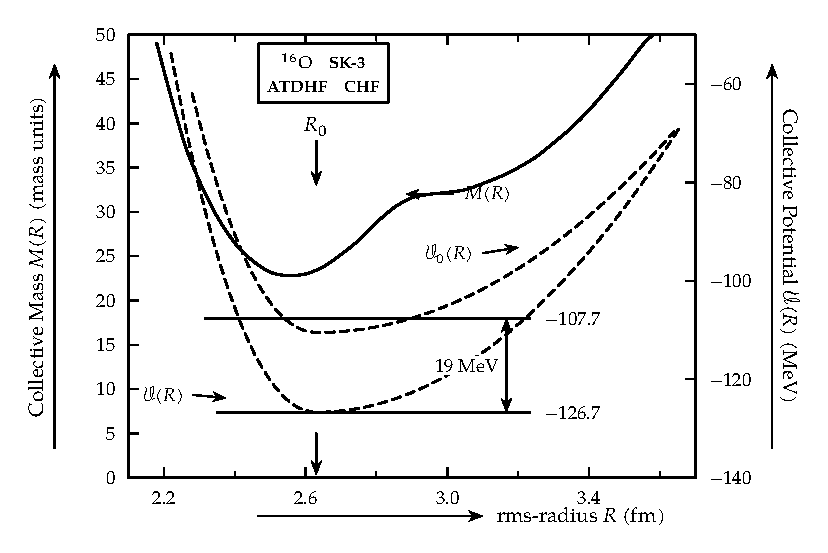
\includegraphics[width=0.75\textwidth]{pictures/12_6}
\par\end{centering}
\caption{\label{fig:12.6}ATDHF 理论中 $^{16}\mathrm{O}$ 同位旋标量单极模的势能面与质量参数。（引自
\cite{Go77}）}
\end{figure}

Giannoni 等人 \cite{GMQ76,GQ80} 计算了轻核同位旋标量四极模的质量参数。他们发现对于有效质量 $m^{*}/m\simeq1$
的 Skyrme 力，ATDHF 质量\ref{eq:12.110} 非常接近简单的 Cranking 质量 {[}见\ref{eq:12.147}{]}。事实上可以证明，\ref{eq:12.75a}
中产生 ATDHF 质量（Thouless-Valatin 质量）与 Cranking 质量（Inglis 公式）之差的项 $\Gamma_{1}$
正比于 $1-m^{*}/m$。

\subsection{绝热微扰论与Cranking公式\label{subsec:12.3.7}}

以微观方式导出集体运动惯性参数的最古老方法是所谓的 Cranking 公式。它最初由 Inglis \cite{In54,In56}
在转动情形下引入，我们在 5.4 节中对此进行了详细讨论。Kerman \cite{Ke61} 针对更一般的集体运动导出了类似的质量参数表达式。我们已在
12.3.2 节中看到，如果在动能\ref{eq:12.81} 中忽略自洽势 \ref{eq:12.74} 的时间奇宇称部分 $\Gamma_{1}$，我们将再次获得该公式。

该公式在过去被极为频繁地使用。因此，我们希望在此给出其在绝热微扰论背景下的通常推导 \cite{Wi55,In56,Be61a,Th61a}。为此，我们假设有一个单参数的
Hamilton 量族 $H(q)$，其中 $q$ 为集体坐标，例如描述核形状的形变参数。如果系统以确定的速度 $\dot{q}$
运动，它将由一个确定的时间函数 $q(t)$ 所表征。然而在实践中并不这样做，我们在推导集体 Hamilton 量时也不需要这种时间依赖关系的显式形式。我们仅仅假设运动是缓慢的。

在每个时刻 $t$，亦即对于每个形变 $q$，我们假设具有 Hamilton 量的本征态 $|k\rangle$，即所谓的绝热基底（adiabatic
basis）\cite{No77}：

\begin{equation}
H|k\rangle=E_{k}|k\rangle\label{eq:12.138}
\end{equation}

本征函数 $|k\rangle$ 以及能量都依赖于参数 $q$，从而依赖于时间 $t$。

Schrödinger 方程的精确解 $|\Psi(t)\rangle$：

\begin{equation}
H(t)|\Psi(t)\rangle=\mathrm{i}\hbar\frac{\partial}{\partial t}|\Psi(t)\rangle\label{eq:12.139}
\end{equation}

现在在该基底中展开：

\begin{equation}
|\Psi(t)\rangle=\sum_{k}a_{k}(t)\mathrm{e}^{\mathrm{i}\phi_{k}(t)}|k(t)\rangle\label{eq:12.140}
\end{equation}

为方便起见，我们在该展开中使用时间相关的相位因子：

\begin{equation}
\phi_{k}(t)=-\frac{1}{\hbar}\int^{t}E_{k}(t^{\prime})\,\mathrm{d}t^{\prime}\label{eq:12.141}
\end{equation}

这本质上处理了绝热态 $|k\rangle$ 的平凡振荡相位。将拟设\ref{eq:12.140} 代入 Schrödinger
方程 \ref{eq:12.139} 并左乘矢量 $\langle l|$，我们得到系数 $a_{k}$ 的一组耦合微分方程：

\begin{equation}
\dot{a}_{l}=-\sum_{k}\langle l|\frac{\partial}{\partial t}|k\rangle\mathrm{e}^{\mathrm{i}\phi_{kl}}a_{k}=-\dot{q}\sum_{k}\langle l|\frac{\partial}{\partial q}|k\rangle\mathrm{e}^{\mathrm{i}\phi_{kl}}a_{k}\label{eq:12.142}
\end{equation}

其中 $\phi_{kl}=\phi_{k}-\phi_{l}$。

该方程仍然是精确的。现在在绝热极限下，即对于小速度 $\dot{q}$ 研究它。我们假设系统在 $t=0$ 时处于绝热基态 $|0\rangle$（其中所有低于
Fermi 面的单粒子能级均被填满），初始条件为：

\begin{equation}
a_{k}(t=0)=\delta_{k0}\label{eq:12.143}
\end{equation}

由于 $a_{k}$ 的时间导数正比于 $\dot{q}$，我们预期在所有时刻，对于 $k\neq0$，$a_{k}(t)$
都很小，而 $a_{0}$ 接近于 1，即系统始终保持接近绝热基态。仅存在对更高态的虚激发，这些激发正比于速度并产生惯性。

在此近似下，对于 $l\neq0$ 我们得到：

\begin{equation}
\dot{a}_{l}=-\dot{q}\langle l|\frac{\partial}{\partial q}|0\rangle\mathrm{e}^{\mathrm{i}\phi_{0l}}\label{eq:12.144}
\end{equation}

在附加假设 $\dot{q}$ 和矩阵元 $\langle l|\partial/\partial q|0\rangle$ 与振荡相位
$\phi_{0l}$ 相比仅具有相对微弱的时间相关性下，我们可以对\ref{eq:12.144} 积分，对于 $l\neq0$
得到：

\begin{equation}
a_{l}=\frac{\mathrm{i}\hbar\dot{q}}{(E_{l}-E_{0})}\langle l|\frac{\partial}{\partial q}|0\rangle\mathrm{e}^{\mathrm{i}\phi_{0l}}\label{eq:12.145}
\end{equation}

由此，我们在有一阶微扰论中计算了波函数\ref{eq:12.140} 中依赖于速度的项，现在能够将总能量表示为“集体坐标” $q$
与相应速度 $\dot{q}$ 的函数：

\begin{equation}
E(q,\dot{q})=\langle\Psi(t)|H|\Psi(t)\rangle=E_{0}+\sum_{k\neq0}(E_{k}-E_{0})|a_{k}|^{2}=\frac{1}{2}M(q)\dot{q}^{2}+\mathcal{V}(q)\label{eq:12.146}
\end{equation}

其中势能为：

\begin{equation}
\mathcal{V}(q)=E_{0}(q)=\langle0|H|0\rangle_{q}\label{eq:12.146b}
\end{equation}

惯性参数即为著名的 Cranking 公式：

\begin{equation}
M(q)=2\hbar^{2}\sum_{k\neq0}\frac{|\langle k|\partial/\partial q|0\rangle|^{2}}{E_{k}-E_{0}}\label{eq:12.147}
\end{equation}

利用多体函数 $|k\rangle$ 为 Hamilton 量 $H(q)$ 的本征函数这一事实，我们可以将该公式略作改写：

\begin{equation}
M(q)=2\hbar^{2}\sum_{k\neq0}\frac{|\langle k|[H,\partial/\partial q]|0\rangle|^{2}}{(E_{k}-E_{0})^{3}}=2\hbar^{2}\sum_{k\neq0}\frac{|\langle k|\partial H/\partial q|0\rangle|^{2}}{(E_{k}-E_{0})^{3}}\label{eq:12.148}
\end{equation}

对于简化的 Nilsson Hamilton 量 $H=H_{0}-q\cdot Q$，我们从而得到：

\begin{equation}
M(q)=2\hbar^{2}\sum_{k\neq0}\frac{|\langle k|Q|0\rangle|^{2}}{(E_{k}-E_{0})^{3}}\label{eq:12.149}
\end{equation}

这一推导基于这样一个假设：绝热基底的状态不会随时间急剧变化。在单粒子能级在 Fermi 面处发生交叉的情形下，这一假设显然崩溃了。此时单粒子态从空态变为占有态，或者反之，且相应的两准粒子态的能量差
$E_{k}-E_{0}$ 趋于零。\ref{eq:12.147} 的分母趋于零，使得矩阵元 $\langle k|\partial/\partial q|0\rangle$
产生极大的峰值，从而 Cranking 公式的推导不再具有合理性。

事实上，当系统跨越这样一个交叉点运动时，可能会发生它不再保持在绝热基态中的情况。这在两个能级 $\epsilon_{1}$ 和 $\epsilon_{2}$
的孤立交叉点处最容易研究，设相互作用矩阵元为 $V_{12}$（两能级之间最接近的距离为 $2V_{12}$）。在此情形下，\ref{eq:12.142}
约化为两个耦合微分方程构成的系统。对于恒定速度 $\dot{q}$ 以及能级 $\epsilon_{1,2}$ 对 $q$ 的线性依赖，该问题可以解析求解。对于系统在赝交叉处跃迁到上层能级的几率
$P=|a_{2}(\infty)|^{2}$，我们得到 Landau-Zener 公式 \cite{La32,Ze32}：

\begin{equation}
P=\exp\left(-\frac{2\pi V^{2}_{12}}{\hbar|\dot{q}||(\mathrm{d}/\mathrm{d}q)(\epsilon_{1}-\epsilon_{2})|}\right)\label{eq:12.150}
\end{equation}

当速度增加时，该几率变大；同样地，当两能级斜率差增加时几率也变大，因为在这些情形下交换两能级性质的相互作用区域相当短暂。在该模型精确公式\ref{eq:12.150}
中，我们发现函数 $P$ 对小速度 $\dot{q}$ 表现出非解析行为 \cite{Sch77a}。通过将\ref{eq:12.142}
按 $\dot{q}$ 展开来求解（其最低阶给出了 Cranking 公式\ref{eq:12.147}），因此可能对应于一种渐近展开。

迄今为止，在何种情况下绝热近似崩溃在某种程度上仍是一个悬而未决的问题。如果使用严格的自洽计算（如 12.3.4 节所讨论的那样），该图景与在固定唯象势阱中的计算大不相同。由于在自洽场中对单粒子能级交叉的避免，绝热条件通常能够得到更好的满足。另一方面，在重离子反应中，速度通常很大，必须考虑越过能级交叉的跃迁。
